%% The options are (you can only choose one from each group):
%%
%% 10pt, 11pt, 12pt: chooses the point size for the document. "11pt" is the
%%                   default.
%%
%% oneside, twoside: whether you want your document onesided or twosided. Note
%%                   that twosided is not guaranteed to work, and style
%%                   guidelines prohibit double sided printouts on final
%%                   copy. "oneside" is the default.
%%
%% draft, final: when printing drafts you can save a lot of paper by using the
%%               "draft" option. It switches to single spacing, displays overful
%%               hboxes with a black box, prints a version number on title page 
%%               and omits signature page. Of course for the final copy make
%%               sure to use the "final" option! "final" is the default.
%%
%% thesis, dissertation: switches between the style for a master's thesis and a 
%%                       Ph.D. dissertation. The differences are fairly minor
%%                       and limited to the front matter. "thesis" is the
%%                       default.
%%
%% actual, proposal: switches between actual document and proposal mode. In
%%                   proposal mode: the title page is simplified, the
%%                   version number is always printed, and the signature page
%%                   is omitted.
%%
%%% Load the new uhthesis document class
%\documentclass[11pt,final,dissertation,actual,subfigure]{uhthesis}
\documentclass[11pt,final,dissertation,actual,subfigure]{uhthesis}

%% hyperref package complains if this isn't here. Might be unneeded when
%% I switch to the new UH thesis style
%\paperheight = 11in

%% Switch to Times font
%\usepackage{times}
\renewcommand{\rmdefault}{ptm}

%%% Load some useful packages:
%% LaTeX2e graphics support
\usepackage{graphicx}
%%	using final option to force graphics to be included even in draft mode
%\usepackage[final]{graphicx}
%% Tell graphicx the default directory for all figures
\graphicspath{{figures/}}

%% Enable subfigure support
\usepackage{subfigure}

%% Provide longtable support, so tables can span multiple pages
\usepackage{longtable}

%% This is a patch of the original longtable package that I stumbled upon
%\usepackage{ltabptch}

%% Make pretty shaped paragraphs
\usepackage{shapepar}

%% Make subsubsections numbered and included in ToC
\setcounter{secnumdepth}{3}
\setcounter{tocdepth}{3}

%% Package to linebreak URLs in a sane manner.
\usepackage{url}

%% Define a new 'smallurl' style for the package that will use a smaller font.
\makeatletter
\def\url@smallurlstyle{%
  \@ifundefined{selectfont}{\def\UrlFont{\sf}}{\def\UrlFont{\small\ttfamily}}}
\makeatother
%% Now actually use the newly defined style.
\urlstyle{smallurl}

%% Define 'tinyurl' style for even smaller URLs (such as in tables)
\makeatletter
\def\url@tinyurlstyle{%
  \@ifundefined{selectfont}{\def\UrlFont{\sf}}{\def\UrlFont{\scriptsize\ttfamily}}}
\makeatother

%% Provides additional functionality for tabular environments
\usepackage{array}

%% Adds new functionality for tables
\usepackage{tabularx}

%% Create a variable width hrule. From:
%% http://tex.stackexchange.com/a/3447/22230
\makeatletter
\def\hlinewd#1{%
\noalign{\ifnum0=`}\fi\hrule \@height #1 %
\futurelet\reserved@a\@xhline}
\makeatother

%% Set up to create an index
%\usepackage{makeidx} 
%\makeindex

%% Puts space after macros, unless followed by punctuation
\usepackage{xspace}

%%% Personal macros
%% Hawai`i with okina
\newcommand{\Hawaii}{Hawai`i\xspace}
%% Hawai`ian with okina
\newcommand{\Hawaiian}{Hawai`ian\xspace}
%% Manoa with kahako
\newcommand{\Manoa}{M\=anoa\xspace}

%% Provides customization of lists
\usepackage{enumitem}

%% Now define question list type
\newlist{question}{enumerate}{1}
\setlist[question]{resume, label=\textbf{\arabic*.}}

%% Define multiple choice answer list type
\newlist{answer}{enumerate}{1}
\setlist[answer]{label=\alph*)}

%% Provides some useful symbols such as checkboxes, circles
\usepackage{wasysym}

%% Define checkbox answer list type
\newlist{checkbox}{itemize}{1}
\setlist[checkbox]{label=\Square}

%% Define radio button answer list type
\newlist{radiobutton}{itemize}{1}
\setlist[radiobutton]{label=\Circle}

%% Allows insertion of fixme notes for future work
%% Note, remove status=draft when printing final version!
\usepackage[footnote, nomargin, status=final]{fixme}
%\usepackage[footnote, nomargin, status=draft]{fixme}
%% turned off marginclue because it generates hbox overflows for each note :(
%\usepackage[footnote, nomargin, marginclue, status=draft]{fixme}

%%% Make URLs clickable
%% Colored links, best for reading PDF on computer
\usepackage[colorlinks, citecolor=blue, bookmarks=true]{hyperref}
%% Colored links and backreferences, for reading PDF on computer
%\usepackage[colorlinks, citecolor=blue, bookmarks=true, backref]{hyperref}
%% Turn off link coloring when printing black & white
%\usepackage[bookmarks=true]{hyperref}

%% Make \autoref from hyperref package capitalize things normally
\def\chapterautorefname{Chapter}
\def\sectionautorefname{Section}
\def\subsectionautorefname{Section}
\def\subsubsectionautorefname{Section}

%% Make links to captions point to the figure, not just the caption at bottom
\usepackage[all]{hypcap}

%% Set up to create a glossary
%\usepackage[toc]{glossaries}
%\makeglossaries

%% Since I'm using the LaTeX Makefile that uses dvips, I need this
%% package to make URLs break nicely
\usepackage{breakurl}

% correct bad hyphenation here
\hyphenation{strong-ly}

%% Useful if you just want to create a PDF of one include file
%\includeonly{appendix-actions}

%%% End of preamble
\begin{document}

%%% Declarations for Front Matter. Capitalize all of these values
%%% "normally". This allows the document class to format them properly.
%% Full title of thesis or dissertation, capitalized like a title should be.
\title{Software Trajectory Analysis: an empirically based method for automated software process discovery}
%% Your name, capitalized normally. Do not include any titles like Dr.
\author{Pavel Senin}
%% Month in which you intend to receive your degree (i.e. graduation).
%% Presumably this will be one of: May, August, or December.
\degreemonth{-}
%% Year of expected graduation.
\degreeyear{2013}
%% Type of degree to be conferred.
\degree{Doctor of Philosophy}
%% This is the chairperson of your committee. Do not use titles like Dr.
\chair{Philip M. Johnson}
%% The other members of your committee, seperated by "\\". Again, no titles,
%% and it is customary to list the outside committee member (if you have one)
%% last.
\othermembers{Kyungim Baek\\
Guylaine Poisson\\
Henri Casanova\\
Daniel Port}
%% The field in which you are obtaining your degree, capitalized normally.
\field{Computer Science}
%% 4-6 optional keywords/phrases for use in indexing or as search terms
%\keywords{software process, time series classification, data mining, knowledge discovery}

%% The version number of your document. Consistent use of this will enable you
%% to tell old drafts from new ones. Final actual documents omit this
%% automatically so you can use it without fear of submission problems at the
%% end. If you do not define this parameter, it defaults to "1.0.0".
\versionnum{1.0.0}

%%% Create the title page from all the information above. Note that the
%%% titlepage is outside the front matter.
\maketitle

\begin{frontmatter}

%%% Signature page is no longer included in the manuscript, Form IV replaces it

%%% Create the copyright page
\copyrightpage

%%% Bring in the dedication page from external file
%%%%%%%%%%%%%%%%%%%%%%%%%%%%%% -*- Mode: Latex -*- %%%%%%%%%%%%%%%%%%%%%%%%%%%%
%% thesis-dedication.tex -- 
%% Author          : Robert Brewer
%% Created On      : Fri Sep 25 14:33:09 1998
%% Last Modified By: Robert Brewer
%% Last Modified On: Thu Mar 16 12:03:14 2000
%% RCS: $Id: thesis-dedication.tex,v 1.3 2000/03/17 21:26:34 rbrewer Exp $
%%%%%%%%%%%%%%%%%%%%%%%%%%%%%%%%%%%%%%%%%%%%%%%%%%%%%%%%%%%%%%%%%%%%%%%%%%%%%%%
%%   Copyright (C) 1998 Robert Brewer
%%%%%%%%%%%%%%%%%%%%%%%%%%%%%%%%%%%%%%%%%%%%%%%%%%%%%%%%%%%%%%%%%%%%%%%%%%%%%%%
%% 

\begin{dedication}

%% Maybe a Kukui Cup logo outline?

  \null\vfil
  {\large
    \begin{center}
      \heartpar{To Yuka: thanks for all the love, support, and patience you
        have shown me while I worked on my Ph.D. It is most deeply appreciated.}
    \end{center}}
  \vfil\null

\end{dedication}


%%% Bring in the acknowledgements section from external file
\begin{acknowledgments}

This research project could not have been completed without the help of a number of people. My deeply thanks go to Prof. Philip Johnson, who has been my most respectful advisor and mentor for my four fruitful years in the Collaborative Software Development Lab. 
  
I'd also like to thank past and present members of CSDL in chronological order: Robert Brewer, George Lee, Michelle Kat\-chuck, Carleton Moore and Jordan Takayama. Special thanks go to George Lee, who developed the initial version of Makahiki. The Makahiki research project would not have happened without your long hours and hard work.

I would like to thank my committee members Prof. David Chin, Prof. Scott Robertson, Prof. Lipyeow Lim, and Prof. Daniel Port for taking the time to read and evaluate this dissertation.

This research is supported in part by grant IIS-1017126 from the National Science Foundation and the funding from the Center for Renewable Energy and Island Sustainability (REIS).

\end{acknowledgments}


%%% Bring in the abstract section from external file
%%%%%%%%%%%%%%%%%%%%%%%%%%%%%% -*- Mode: Latex -*- %%%%%%%%%%%%%%%%%%%%%%%%%%%%
%% uhtest-abstract.tex -- 
%% Author          : Robert Brewer
%% Created On      : Fri Oct  2 16:30:18 1998
%% Last Modified By: Robert Brewer
%% Last Modified On: Fri Oct  2 16:30:25 1998
%% RCS: $Id: uhtest-abstract.tex,v 1.1 1998/10/06 02:06:30 rbrewer Exp $
%%%%%%%%%%%%%%%%%%%%%%%%%%%%%%%%%%%%%%%%%%%%%%%%%%%%%%%%%%%%%%%%%%%%%%%%%%%%%%%
%%   Copyright (C) 1998 Robert Brewer
%%%%%%%%%%%%%%%%%%%%%%%%%%%%%%%%%%%%%%%%%%%%%%%%%%%%%%%%%%%%%%%%%%%%%%%%%%%%%%%
%% 

\begin{abstract}
Abstract goes here, and will be written once the proposal is mostly done.
\end{abstract}


%%% Generate list of FiXmes, will be silent in final mode
\listoffixmes

%%% Generate table of contents
\tableofcontents

%%% Generate list of tables
\listoftables

%%% Generate list of figures
\listoffigures


\end{frontmatter}

%%% Include each chapter
% my main text chapters
\chapter{Introduction}\label{chapter_introduction}
\textit{The central issue I address in the dissertation is a possibility of recurrent behaviors discovery from 
publicly available software process artifacts by leveraging data mining and knowledge discovery techniques. 
In particular I explored an approach of discovering of recurrent behaviors through the mining of time series that
are constructed by temporal ordering of measurements extracted from software process artifacts.
Further, I shall propose a novel technique for characteristic patterns discovery from time series and show its 
applicability to the problem at hands.}

\textit{The problem's background is provided in the Section \ref{section_background}. 
Section \ref{section_software_process_design} presents classical approaches for software process design and shows its limitations.
Section \ref{section_research_hypothesis} introduces the research hypothesis.
Section \ref{knowledge_discovery} provides a background into the problem of knowledge discovery 
from time-series.
Section \ref{section_trajectory_definition} connects two problems and provides definitions.
Section \ref{section_contributions} enumerates main contributions of the thesis, 
while section \ref{section_organization} explains the thesis organization.}

%
% >> section
%
\section{Background}\label{section_background}
Contemporary software projects concern with development of complex software systems and typically have 
a considerably long life-cycle - well over decade.
A project's development and maintenance activities are usually carried out by geographically 
distributed teams and individuals. The development pace, the experience, and the structure of the 
development team continuously change with project progression and as developers joining and leaving. 
When combined with schedule and requirements adjustments, these create numerous difficulties 
for developers, users, and stakeholders, ultimately affecting the project success \cite{citeulike:2207657}. 

This software development complexity phenomena was identified in 1968 as ``Software crisis'' 
\cite{naur_crisis_68}, and was addressed by bringing the research and the practice of software development 
(or as it was called ``programming'') under the umbrella of Engineering - in an effort to provide 
the control over the process of software development. 
Following the engineering paradigm, numerous methodologies and models of software design and development 
process, known as \textit{software processes}, were proposed \cite{citeulike:10002165}.

\begin{defn}\label{def_process}
A \textbf{\textit{Software Process}} defines a sequence of activities performed in order 
to design, develop, and maintain software systems.
\end{defn}
Examples of such activities include requirements collection and creation of UML diagrams, 
requirements testing, code development,  testing, etc. The intent behind a software process is 
to provide a control over software evolution by implementing a global strategy and by structuring
and coordinating human activities in order to achieve the goal - deliver a functional software system 
on time and under the budget. 

Since then, much research has been done on software processes resulting in a number
of software development models and paradigms. Some of these were widely accepted by practitioners 
and evolved into industrial standards for software development processes such as CMM, ISO, PSP, 
and others \cite{citeulike:5043104}. However, in spite of this effort, industrial software 
development remains error-prone and more than half of all 
commercial software development projects ending up failing or being very poorly executed 
(Rubinstein, ``Chaos Reports'', 2006) \cite{chaos2006}. Some of them are abandoned due to running 
over budget, some are delivered with such low quality, or so late, that they are useless, and some, 
when delivered, are never used because they do not fulfill requirements. 

Through the analyses of software project failures, it was acknowledged, that the engineering 
paradigm might not be the best way to provide a control over software development processes 
(\cite{citeulike:3729379} \cite{citeulike:5203446}) due to the fact that Software engineering 
is dealing with significantly different from other Engineering fields problems \cite{citeulike:2207657} .
The chief argument supporting this point of view is the drastic difference in the cost model:
while in Software Engineering there is almost no cost associated with materials and 
fabrication, these usually dominate cost in all other Engineering disciplines, but, 
ironically, Software Engineering is suffering from the costs and challenges associated with 
continuous re-design of the product and its design processes - the issue which is 
hardly seen at all in other Engineering areas. 
Further, it was found, that most of the engineering-like models are rigid, ``context-free'',
and rather prescriptive, i.e. they are universally defined independently of a particular 
organizational structure or a project specificities \cite{sacchi_2001}, and while they 
structure processes and provide the control, following them does not guarantee the success.
Yet another argument supporting alternative to engineering approaches is the increasing 
understanding and appreciation of a human role in software development processes over tools, 
technologies, and standards \cite{citeulike:6580825} \cite{citeulike:149387}
\cite{1605185} \cite{citeulike:113403} \cite{1605188} \cite{citeulike:12743107}. 

Along with Software Engineering, a number of alternative, flexible and user-oriented software processes 
emerged from academy, hobbyists, and practitioners addressing aforementioned issues \cite{citeulike:3729379}. 
Among others, the Free/Libre/Open-Source Software model (FLOSS) and the software craftsmanship  
approaches gained a significant credibility in community. 
While the former \textit{holistic} software process paradigm emphasizes loosely-organized 
collaboration, frequent releases, and effectively removes the boundary between developers 
and customers, the latter, human-centric approach, is built upon the roles of highly 
motivated skilled individuals \cite{citeulike:262020} \cite{citeulike:2759198}. 

Nevertheless, alternative processes were found to be plagued by the same complexity issues. 
As it was shown, most of FLOSS projects never reach a ``magic'' 1.0 version \cite{citeulike:12480029}. 
Among others, the great "infant mortality rate" of FLOSS projects was related to a burnout, 
inability to acquire a critical mass of users, loss of leading developer(s), and forking \cite{richter2007critique}. 
Software craftsmanship, from other hands, not only challenges developers with technological advances 
requiring continuous skills improvement, but creates significant cost and effort estimation difficulties for
stakeholders and project managers \cite{citeulike:11058784}. However, despite to these issues, 
the alternative processes proved that the disciplined manner of programming and the modularization  
of the software are capable of delivering large and reliable software systems, most notable Linux OS,
suggesting that community-driven processes as good as industrial engineering-like processes.

Currently, it is widely acknowledged, that there exists no single ``silver bullet'' process which 
can bring a software development project to success \cite{citeulike:1986013}. 
Processes are numerous, each has advantages and drawbacks, and each is accompanied with 
numerous application recommendations, success stories, and with failure experiences. Nevertheless,
the alarming rate of failing projects suggests that our understanding of software process ``mechanics''  
is limited and insufficient\cite{citeulike:12550665}. 
The enormous cost of the lost effort, measured in hundreds of billions of US dollars 
\cite{citeulike:2207657} \cite{citeulike:2207653} \cite{citeulike:2207655}, 
continues to provide motivation for further research on software processes. 

%
% >> section
%
\section{Software process design}\label{section_software_process_design}
Traditionally, approaches to software process design and improvement are divided into two distinct categories. 

The first category of software process design approaches consists of traditional to engineering 
\textit{top-down} prescriptive techniques through 
\textit{proposing a process based on specific patterns of software development}. 
For example, the Waterfall Model process proposes a sequential pattern in which developers first create a 
Requirements document, then create a Design, then create an Implementation, and finally develop Tests. 
The Test Driven Development process, from other hands, proposes an iterative behavioral pattern in which
the developer must first write a test case, then write the code to implement that test case, then re-factor the 
system for maximum clarity and minimal code duplication \cite{citeulike:6086365}. 

While the top-down approach follows the usual path of trials and errors, and seems to be an extension 
of natural to humans creative processes of invention and experimentation, 
the ``invention'' of an adequate to the task software process is far from trivial 
\cite{citeulike:5043104} \cite{citeulike:1986013}. Moreover, an evaluation cycle of an invented process
is usually very expensive and considerably long.
In addition, it was shown that the process inventors are often limited in their scope and tend to assume 
idealized versions of real processes, thus, often produce ``paper lions'' - process models which are 
likely to be disruptive and unacceptable for end users, at least in their proposed form 
\cite{citeulike:9758924}, which creates a large discrepancy between actions that supposed to be done for 
the novel process and what was actually performed by particular individual or the team.

The second category of software design approaches consists of \textit{bottom-up} techniques 
that focus on a \textit{performed process reconstruction through noticing of recurrent development 
events and behaviors} or as it also called \textit{process enactment}. 
Usually, the process reconstruction task is viewed as a two-levels problem where the first level 
consists of a patterns discovery (segmentation) while the second level consists of patterns recognition 
and their network analysis \cite{citeulike:2703162}.
One of the first works in this category was by Cook and Wolf, where they show a
possibility of automated extraction of a process model through the mining of recorded 
process event logs \cite{citeulike:328044} \cite{citeulike:5120757} \cite{citeulike:5128143}. 
Later work by Huo et al. shows that it is also possible to improve an existing process
through the event logs analysis \cite{citeulike:7691059} \cite{citeulike:7690766}. 

While the bottom-up approaches seem to be more systematic and potentially less complex than invention, 
they also affected by a number of issues. A chief among these is the observability issue - 
it is usually very difficult to conduct a full depth study on a live project due to the privacy concerns. 
Moreover, it is expensive to observe a process performed by a team for a whole life-cycle of a project. 
Yet another issue is the capacity of currently available process discovery techniques - 
typically these need to be supervised by experts and finely tuned in order to reconstruct 
distributed and concurrent processes. 

Nevertheless, despite to their differences, both techniques for software process design are 
producing process models that effectively are the series of actions that must be performed successively 
(sequentially and sometimes iteratively) in order to deliver a software. 
In order to produce the viable model, the ``process inventors'' put the best of their knowledge, experience,
creativity, and logical reasoning into the proposed sequence of steps, while ``process re-constructors 
strive to eliminate the noise and to converge to a concise process model that is supported by the 
majority of observations. 
This attention to synthesis of sequential steps, leaves other phenomenas, such as team's structure, work schedule, 
developer's discipline, their behaviors, and motivation behind. While this issue was recognized previously
and resulted in a number of studies which called for attention of human element in software production 
\cite{citeulike:149387} \cite{citeulike:113403} \cite{citeulike:205322} \cite{citeulike:12798652}, 
it is still largely ignored in industrial practices \cite{citeulike:12798659}, mostly due to the 
difficulties in benefit estimation \cite{citeulike:12798662} \cite{csdl2-12-11}.

%
% >> section
%
\section{Free/Libre Open Source processes}\label{floss_processes}
Along with growing amount of publicly available software, it became obvious, that self-organizing communities of 
mostly ``recreational'' software developers and active users are capable to successfully manage large code base, 
but to deliver software increasingly complex and surprisingly popular.
Many of large, ``global'' open source software development projects, such as Linux and its derivatives, 
Gnome, Apache HTTP Server, MySQL, and others, not only have comparable with industrial projects development team 
and code-base sizes, but the same average defect rate \cite{coverity2012}. 
These facts have attracted a considerable attention from industry and many organizations 
seek to emulate successful open source software processes in traditional ``closed source'' environment 
\cite{oss_virtual_organizations} \cite{oss_balance} \cite{oss_hp} \cite{oss_4industry}. 

\begin{figure}[ht!]
   \centering
   \includegraphics[width=140mm]{figures/Linus.Kernel.ps}
   \caption{A Torvald's response suggesting that practical reasons, the ``real-life'', should be always considered 
   over specifications.
   Excerpt from the Linux mailing list. \url{http://lkml.indiana.edu/hypermail/linux/kernel/0509.3/1441.html}}
   \label{fig:kernel}
\end{figure}

If we consider this as an assertion that open-source software processes are at least as good as engineering-like 
software process models, then, the freely available open-source process software artifacts potentially bear an 
incredible wealth of the information worth of studying. Moreover, the striking differences of open-source processes 
from a traditional software development could potentially reveal novel software processes and their aspects that 
were previously not accounted for. 
For example, consider that the most significant document in industrial software processes - a specification - 
is rarely considered at all in open source world. In FLOSS projects the software look and its functionality are 
rather viewed as open-end questions. Even in the Linux kernel development, which is probably one of the few strictly 
moderated FLOSS development processes, developers prise practical reasons over specifications 
\ref{fig:kernel}.

Yet another source of motivation for studying of public FLOSS software process artifacts comes from the fact that 
in order to facilitate the distributed FLOSS software development processes, the community is highly encouraging
developers to commit their changes rather often \cite{so-checkin} \cite{git-best-practices1}.
The frequent commits and the changes visibility practice is often cited as vital for health of software 
process as mentioned in some lengthy discussions: ``\textit{Don't Go Dark}'' \cite{checkin-dgd-2008}, 
``\textit{Check In Early, Check In Often}'' \cite{checkin-ch-2012}. Potentially, frequent commits create artifacts 
trails that provide finer resolution into project development and allow more thorough process recovery.

%
% >> section
%
\section{Public software repositories}\label{section_public_repositories}
Recently, the aforementioned situation changed, and the interest for process enactment and reconstruction, 
as well as attention to the human-specific components of software processes has been revived. 
This change is driven by the increase in public data that are made available by the proliferation of open 
source communities.

Currently, with accessible personal computers, friendly software development toolkits, and due to massification
of the use of the web as
a platform for collaborative work, small-scale commercial and recreational 
programming become very popular. 
Today, free code hosting sites such as SourceForge, GoggleCode, and GitHub host thousands of 
Free/Libre Open Source Software (FLOSS) projects.
These publicly offer numerous software artifacts such as design documents, source codes, bugs and issue records, and 
developers and users communications.
Further, Q\&A and social websites for developers such as StackOverflow, Biostars, TopCoder and others becoming 
increasingly popular among the software developers as places for exchanging experiences, learning new tricks, and 
improving skills, plus, they offer anonymized data back to the community.

The public availability of numerous software process artifacts effectively removes not only the high cost of observation, 
but most of the privacy concerns - the two issues that previously made any large-scale analysis of software projects 
unfeasible for most researchers.

Scientific community response on the availability of public artifacts was overwhelming, and a number of 
venues was established addressing the increased interest. 
Since 2004, the International Conference on Software Engineering (ICSE) hosts a Working Conference on 
Mining Software Repositories (MSR). The original call for papers stated MSR's purpose as 
\textit{``... to use the data stored in these software repositories to further understanding of software 
development practices ... [and enable repositories to be] used by researchers to gain empirically based 
understanding of software development, and by software practitioners to predict and plan various aspects 
of their project''} \cite{msr2004} \cite{citeulike:7853299}. 
Several other venues: International Conference on Predictive Models in Software Engineering \cite{promise12}, 
International Conference on Open Source Systems, the Workshop on Public Data about Software Development, 
and the International Workshop on Emerging Trends in FLOSS Research have also played
an important role in shaping and advancing this research domain.

Some of the published work addresses the software process discovery. Among others, most notable and 
relevant to my research is work by Jensen \& Scacchi. In their early work, they demonstrated, that 
information reflecting software processes can be gathered from public systems \cite{citeulike:12550640}. 
Later, in \cite{citeulike:5043664} and \cite{citeulike:5128808}, they show, that by manual mapping of 
collected process evidence to a pre-defined process meta-model it is possible to reconstruct some 
of the FLOSS processes. 
Another closely related to my research is work by Hindle et al. where they has shown that it is possible to 
discover software process evidence through partitioning \cite{citeulike:10377366}.

However, the research work based on mining of software process artifacts shows, that while public availability 
of artifacts is minimizing observability and privacy issues, the nature of these artifacts creates a number of 
challenges which I discuss in the chapter X, which limit the possible scope of the research and significantly 
elevate the complexity of the process discovery effectively rendering previously designed techniques inefficient.
Thus, the novel analysis and discovery techniques are needed to be developed for public software process artifacts 
analysis \cite{citeulike:7853299}.
% when ``\textit{... going beyond code and bugs...}'' 

%
% >> section
%
\section{Research hypothesis, scope of the dissertation}\label{section_research_hypothesis}
In previous sections, I have outlined the evidence of a limited performance of existing engineering-like 
software processes (Section \ref{section_background}),
as well the oversight of a variety of human factors that fall beyond a typical sequence of development 
actions by traditional approaches to software process design (Section \ref{section_software_process_design}).
Then, I have identified a few differences of FLOSS processes from traditional Software Engineering 
(Section \ref{floss_processes}), which can potentially shed light on human-driven aspects of software development.
Finally, I have pointed out a growing wealth of publicly available software process artifacts 
(Section \ref{section_public_repositories}) that is worth to explore for a better understanding not only 
FLOSS software processes, but their human factors. All this provided a motivation to my exploratory study, 
whose details I outline in this section.

In my work, I attempted to explore the possibility of discovery of a specific human-driven aspect in 
FLOSS software development that is a \textit{\textbf{behavior}}, which I define as the mannerism in which a 
developer, or a team, conduct their everyday work. 
In particular, I explore the possibility of discovery of \textit{recurrent behaviors}, i.e. behaviors supported 
by a numerous evidence, from software process artifacts. 

For example, if within an observation interval one developer frequently runs unit tests before committing 
changes into repository, while another usually commit changes without running the tests, the first developer's
habit of testing a code before the commit is a recurrent behavior that may reflect the developer's discipline,
or an unusual attention to some particular part of the code. 
Consider another example, if one of the developers usually commits code changes in mornings, while another 
developer late in the day, these two recurrent behaviors, might indicate a constraints that are put on the 
project, or the process, or on the developers themselves.
Obviously, latter behaviors should be possible to quantify by simple analysis of commit timestamps, while 
the former can be discovered by the analysis of co-occurring changes in the source code. 
Moreover, these and similar recurrent behaviors could be further associated with certain project's or process 
traits, such as pace, agility, size, complexity, code quality and others, which will not only extend our 
knowledge of human factors in software processes, but will lay a foundation for future research in software 
processes.

To begin with, I hypothesized, that \textbf{\textit{it is possible to discover recurrent behaviors from 
publicly available software process artifacts}}. 

Following the hypothesis, I have investigated a number of publicly available software repositories,
their artifacts, and a number of applicable data-mining techniques in a preliminary exploratory study 
\cite{csdl2-10-09}. However, similarly to other studies in the field, I have discovered, that while FLOSS 
process artifacts are numerous and readily accessible, their irregular, snapshot-like nature and the poor 
informational content significantly limit the applicability of known techniques for process mining.

In order to overcome this issue, I have casted the initial problem of event-based recurrent behaviors 
discovery into more generic problem of knowledge discovery from time series and approached it
by developing a novel technique for interpretable comparative analysis of time series that allows 
characteristic patterns discovery and ranking called SAX-VSM \cite{sax-vsm}. 

Further, I have developed a software artifacts analysis framework, called Software Trajectory Analysis, 
which aids in software artifacts collection, software process and product evolutionary metrics extraction, 
and their comparative analyses that enable discovery and ranking of characteristic patterns.


 in rank highlight is  transformation into  and by using I approached the problem of knowledge discovery 

developed a 
software process artifacts mining framework called Software Trajectory Analysis which is built upon 
a novel technique for comparative analysis of time series that allows characteristic patterns discovery 
and ranking.

This dissertation presents its results, as well as introduces a novel data mining technique designed to 
alleviate difficulties with interpretability of quantitative results obtained through mining of software
artifacts trails. 

%
% >> section
%
\section{Knowledge discovery from time series}\label{section_knowledge_discovery}
In data mining, time series are used as a proxy representing a vast variety of real-life phenomena 
in wide range of fields including, but not limited to physics, medicine, meteorology, 
music, motion capture, image recognition, signal processing, and text mining. 
While time series usually directly represent observed phenomenas by capturing their measurable evolution in time, 
the pseudo time series often used for representation of various high-dimensional data 
by combining data points into ordered sequences. 
For example in spectrography data values are ordered by component wavelengths \cite{citeulike:12550833};
in shape analysis the order is the clockwise walk direction starting from a
specific point in the outline \cite{citeulike:12550835}, in image classification the numbers of pixels
are sorted by color component values \cite{citeulike:2900542}.

Many important problems of knowledge discovery from time series reduce to the core task of finding 
characteristic, likely to be repeated, sub-sequences in a longer time series. 
In the early work these were called as 
\textit{frequent patterns} \cite{citeulike:5159615}, 
\textit{approximate periodic patterns} \cite{citeulike:1959582},
\textit{primitive shapes} \cite{citeulike:5898869}, 
\textit{class prototypes} \cite{citeulike:4406444}, 
or \textit{understandable patterns} \cite{citeulike:3978076}. 
Later, similarly to Bioinformatics, these were unified under the term \textit{motif} \cite{citeulike:3977965}.
Once found, motifs can be used for a hypothesis generation by finding their associations with known,
or unknown phenomenas \cite{citeulike:3977965}. 

The recent advances in semi-supervised and unsupervised finding of such characteristic sub-sequences, 
in particular work based on \textit{shapelets} \cite{citeulike:7344347} \cite{citeulike:11957982}
\cite{citeulike:12552293} and \textit{bag of patterns} \cite{citeulike:10525778}, show a great potential 
of application of time series data-mining techniques to a wide variety of high-dimensional data.

Unfortunately, both techniques provide a limited insight into the data and suffer from performance issues. 
While exact shapelet techniques allow discovery of class-characteristic patterns and facilitate classification,
algorithm is almost quadratic and provides limited insight into class specificities. 
The bag of patterns algorithm, while performs in a linear time, requires a previous knowledge for input parameters 
selection and does not offer class generalization.

In order to overcome this limitations, in this thesis I propose a novel approach for time-series classification and 
knowledge discovery that is called SAX-VSM and is based on symbolic approximation of time series and vector space model. 
As I shall show, SAX-VSM is capable to discover and to rank characteristic subsequences representing time series classes. 
The proposed algorithm not only facilitates classification, but provides insights into the both: classification results 
and time series classes specificities. As I shall show, by facilitating the class' characteristics patterns ranking,
SAX-VSM enables the discovery of recurrent behaviors and their heat-map like visualization. 

\section{Software trajectory analysis}\label{section_trajectory_definition}
Previously, Johnson et al. defined \textit{software metrics telemetry streams} \cite{citeulike:12550871}, 
(what they re?) and showed, that it is possible to improve software development process by using the 
knowledge extracted by experts through visual analysis of these streams.
 
Similarly to software metrics telemetry streams, I abstract software process artifact by collecting their 
metrics and arrange these measurements by artifact creation time into high-dimensional vectors. 
These non-equidistant, often sparse and uneven in length time series 
I call ``\textbf{software trajectories}''. Similarly to approximate trajectories of objects in 
a physical space, or reduced in complexity sequence of states of a dynamic system (Poincare' maps), 
the \textit{software trajectory is a curve that describes a software project progression in a space 
of a chosen metrics}.

Through an exploratory study, I have discovered, that by the comparative analysis of software trajectories 
with SAX-VSM it is possible to discover and to interpret recurrent behaviors. This workflow that 
consists of software artifacts collection, their metrics extraction, and comparative analyses I call 
\textit{\textbf{Software Trajectory Analysis}} (STA). 

In this thesis, through three case studies, I will show, that Software Trajectory Analysis is capable 
of discovering of a various characteristic patterns which ca be associated with recurrent behaviors.

\section{Contributions}\label{section_contributions}
Main contributions of my work can be summarized as follows: 
\begin{itemize}
\item I propose a novel, generic algorithm for interpretable time series classification: SAX-VSM. 
While the classification performance of this algorithm is at the level of current state of the art, 
it offers an outstanding feature - discovery, generalization, and ranking of class-characteristic features. 
This, in turn, enables knowledge discovery by offering much clearer insight into classification results than any of 
competing techniques.
In addition, SAX-VSM is very fast in classification and has a small memory footprint. 
Overall, I expect this algorithm to play an important role in future because of the growing ubiquity of time series and 
a growing interest in behaviors.
\item Powered by SAX-VSM, I design a Software Trajectory Analysis (STA) framework, and through case-studies 
show its capacity for recurrent behaviors discovery from publicly available software process
artifacts. While case studies are obviously limited, I argue that STA is a useful knowledge discovery tool applicable for a 
variety of software process artifacts and metrics. 
\item Finally, I provide SAX-VSM and STA implementations to community.
\end{itemize}

\section{Dissertation Outline}\label{section_organization}
The rest of this dissertation is organized as follows. Chapter \ref{chapter_background_work} discusses the history 
of Software Engineering, previous work in software process discovery, mining of software repositories, and current 
state of the art in time series mining. Chapter \ref{chapter_sax_vsm} proposes an algorithm for interpretable 
time series classification. Chapter \ref{chapter_sta} discusses the design of STA framework and presents case studies.
Chapter \ref{chapter_conclusions} concludes and discusses several directions for future study.
%
%\section{Research problem statement and Scope of the dissertation}
Software is coded by humans. Whether in team or individually, humans perform relevant 
daily activities in order to reach the goal - deliver the software. Understanding of these
human activities spanning through the life-cycle of the software, in connection with personal 
and team's motivations, environment settings and constraints essentially enables one to
comprehend the software process. It is worth noting, that roughly \todo[inline]{put here something 
about two components - the human-driven, non-recurrent and creative activity - 
the behavioral component - and the process and the technology/toolkit component which
provides a measurable marginal effect}
\todo[inline]{Here, put stuff about observing the process and artifacts availability}

\todo[inline]{Here, put stuff about time-series analysis flexibility and its difference from 
convenient process mining.}

While it is shown by the large body of previous research, that it is technically possible 
to factor out the impact of the technology and the process, the impact of the behavioral 
component is yet to be studied. Hence, my primary research question is this:
\begin{myindentpar}{0.07\linewidth}
 \textbf{Can we discover recurrent behaviors in software processes from project
  repository artifacts?}
\end{myindentpar}

Obviously, in order to answer this question correctly two interconnected, secondary, question must be resolved:
\begin{myindentpar}{0.07\linewidth}
 \textbf{Which kind of software process artifacts reflect recurrent behaviors?}
\end{myindentpar}
\begin{myindentpar}{0.07\linewidth}
 \textbf{Which data-mining method is sensitive and selective enough to recover recurrent behaviors
from software process artifacts?}
\end{myindentpar}
These two can be broken down further to the problem of studying and classifying of software process artifacts,
methods of their extraction and partitioning, and, of course, the problem of recurrent behaviors discovery.

As was mentioned above, in this thesis I am focusing on a very narrow subject - exploring approaches
for uncovering of recurrent behaviors or ``programming habits'' out of software process artifacts.
While I will show, that, potentially, many software-development activity behaviors can be recovered,
their classification, impact and performance studies are beyond the scope of this thesis.


%
%\section{Organization of the dissertation}
%
%\chapter{Prior and related work}\label{chapter_background_work}
My research focuses on the techniques which aide in the knowledge discovery from a process of 
software development. There is much previous relevant work related to my goal processes; work combines is based on previous research from multiple research areas: software engineering, 
software repository mining, process mining, knowledge discovery from time series,
and information retrieval. 

By extending existing knowldge about software processes and repository mining and combining 
it with a novel technique for knowledge discovery from time series, 
I was able to develop an automated framework for recurrent behaviors discovery from publicly 
available software repositories.

In this chapter I will review previous work relevant to my research.

\section{Engineering in software development}
Since the invention of Charles Babbage’s difference engine in 1822, computers (hardware) 
have required a means of instructing them to perform a specific task. This means is known 
as a programming language. By using programming instructions, software develeopers (programmers)
write the software that is collections of computer data and instructions, which is used by 
users to accomplish specific tasks. The very first software, or more precisely a set of 
instructions implementing a method for calculating a sequence of Bernoulli numbers using 
Charles Babbage's Analytical Engine, was designed by Ada Lovelace in 1942 and predates modern 
computers. 

As time has progressed, computers have made giant leaps in processing power and become 
general-purpose computing devices. Consequently, the variety of software and 
the complexity of its development has grown ``several orders of magnitude'' \cite{naur_crisis_68}. 
This effectively created a number of organizational problems which dominated development of 
early software systems. Among these, historians are mentioning increasing scale of software projects, 
excessive ambition, difficulties in estimating project cost and length, inadequate documentation, 
skimping on design and testing \cite{mahoney_roots_1990} \cite{citeulike:12748733} 
\cite{citeulike:833903}.

All these problems were recognized at the NATO Conference on Software Engineering, held in Garmisch,
Germany in 1968. It worth noting, that before the actual conference, as was pointed by the 
conference proceedings editors, engineering paradigm was chosen without actual plan of actions - 
\textit{``the phrase ``software engineering'' was deliberately chosen as being provocative, in implying 
the need for software manufacture to be [based] on the types of theoretical foundations and practical 
disciplines[,] that are traditional in the established branches of engineering''} \cite{citeulike:12787786}.
At the conference, it was acknowledged, that the increasing complexity of programming 
work had overwhelmed the technical and managerial ability of software teams: software was shipped late,
over budget, worked inefficiently, and was unreliable. Later, while working on the proceedings, the term 
``software crisis'' was coined by the editors in order to describe the desperate state of 
software development and its increasing complexity \cite{naur_crisis_68}.

Nevertheless, the ``software engineering'' idea was provocative enough to shape the minds of researchers 
and practitioners. At large, it was accepted that the software can be successfully ``manufactured'' 
through ``engineering'' - i.e. with the application of a systematic, disciplined, quantifiable approach 
to the design, development, operation, and maintenance. 

Using this paradigm, researchers and practitioners designed a number of software development processes 
providing detailed guidelines on how to reach the goal - deliver the software - efficiently and in time. 
These processes were declared as the means for improvements in terms of quality, speed, and execution cost 
over existing practices. They were studied within academic settings and adopted by industry. 
Some of this processes were further standardized, shaping the best practices of contemporary 
software development \cite{citeulike:9962021}. 

The processes, that I am addressing here, can be found in numerous studies and described at length 
in industrial and academic literature. Too numerous to name, they can be categorized by the level 
of their application:
\begin{itemize}
 \item global organizational standards, like CMMI, ISO 9000, and SPICE. 
 \item large industrial software models, such as Waterfall, Spiral, Cleanroom, etc.
 \item smaller scale, flexible methodologies: FDD, TDD, Pair Programming, etc.
 \item general guidelines and principles aiming to improve the software process flow, 
such as ``build before commit'' and others.
 \item and finally, the processes for improving existing processes of software development 
on the organizational, team, and personal levels: TSP, PSP, Six Sigma, etc.
\end{itemize}
While some of these are products of a ``technology transfer'' - resulted by direct copying or by an 
application of existing engineering principles to software development process (like Waterfall model), 
some, and in particular agile methods, considered to be particular to software-engineering. 

\subsection{Issues with engineering-like processes}
Currently, in Software Engineering, there are numerous software process, models, methodologies, 
and coding conventions exist for any level and any stage of the software development carried out by 
any team size at any project scale. 
This amount of well-grounded and documented knowledge creates an impression, that the area of 
software development process is thoroughly explored, and that there exists a deterministic choice 
for a model and a processes for any given software project leaving almost no doubts in 
its faith - it will be completed according to the specification, in time, and under the budget.

However, it is far from being true - software projects do fail at the considerably high rate and 
many challenges exist in software product development. Many software projects continue to run over 
the budget, do not meet the schedule. Some of the seemingly proper executed projects caused property 
damage \cite{citeulike:11044022}, and a few projects caused loss of life \cite{citeulike:712058}. 
The ``Chaos Report'' from the Standish Group, that only ``35\% of software projects in 2006 can be 
categorized as successful - meaning they were completed on time, on budget and met 
user requirements'' \cite{chaos2006}. These thirty two percent of success clearly manifest that 
it is somewhat illusory statement that we are capable to understand and to control software processes.

This rather poor performance of the mainstream software engineering processes 
ignited a new wave of research in the field in recent decades. Gradually, researchers and 
practitioners alike recognized, that a direct application of classical engineering - that 
excludes a ``human component'' by governing software processes in a top-down fashion 
might be somewhat erroneous. 
Also, it was recognized that over many years, continuous formalization of the field and 
excessive attention to software process metrics may malformed not only the software development 
practices landscape, but education and a professional code of conduct. 
This recognition forced some of the professional associations to review their licensing policies 
\cite{citeulike:11045517} and some educators to change their opinions \cite{citeulike:5203446}. 

\section{Alternative software processes}
In parallel with industrial engineering-like software processes, another phenomena, 
the Free/Libre Open Source Software (FLOSS) development arose and proven its efficiency and effectiveness.
The FLOSS processes are significantly different from typical SE process on many levels:
\begin{itemize}
 \item First of all, FLOSS processes are highly geographically distributed, which significantly contradicts 
 to developers collocation usually assumed by the most of the SE processes. 
 \item Secondly, open-source processes do not explicitly define timeline, developers roles, and 
 the process itself. Typically, the project flow is rarely governed and does not require any sort of 
 documented software process. Most of FLOSS projects accept for review and embed source code from anyone.
 \item Finally, FLOSS delivers software free of charge, promoting its reuse, modification, and redistribution.
 However, mostly due to this, the maintenance and the support are rarely provided.
\end{itemize}

Nevertheless, despite to the apparent lack of the control over the software processes in FLOSS projects, they 
has proven their ability to deliver large in size software systems of high quality for the fraction of cost 
of similar industrial projects.

Most of the success is contributed to the motivation of open source developers.

Lately, third approach to software development emerged - software craftsmanship emerged 
\cite{citeulike:11058561}, \cite{citeulike:11058554}. The followers of this methodology 
are not only focused on the delivering ``well crafted'' software and continuously adding value,
but on the apprenticeship - on forming communities and engaging more people in software development.
While recommendation exists \cite{citeulike:11058784}, little known about the research 
in software craftsmanship and apprenticeship processes.

All this continues to engage thoughts and fuels the search not just for the exact definition 
of software development, but deep, fundamental for efficient processes resolving. 
Is software development an engineering discipline? Is it a craft \cite{citeulike:5203446}? 
Or is it an art \cite{citeulike:11045694}?

Answers to these questions would require extensive interdisciplinary studies to be made, 
but what is obviously clear, is that formal software development process, as an engineering 
is a creative, human activity. 
Whether software is coded 
by team where its members have a variety of skills and experience, or by a single individual,
they all driven by their believes and motivations. While usually developers agree on the use of 
particular technologies, development tools, and a development process with imposed timeline and 
a budget, the software process is - as many other human activities - highly creative and mostly 
non-recurring. Thus, the choice of methodology, technology, or tools provides only a marginal 
effect on this human-based and human-driven process. While this effect can be measured through 
the common approach by using a control environment factoring out human component, the most of 
the difference, which lies in human creativity, motivation and productivity is unknown and yet, 
mostly immeasurable.

\section{Software process discovery}\label{process.discovery} 
Although process mining in the business domain is a well-established field with much software developed up to date (ERP, WFM and other systems), ``Business Process Intelligence'' tools usually do not perform process discovery and typically offer relatively simple analyses that depend upon a correct a-priori process model \cite{citeulike:3718014} \cite{citeulike:5044991}. This fact restricts direct application of business domain process mining techniques to software engineering, where processes are usually performed concurrently by many agents, are more complex and typically have a higher level of noise. Taking this fact in account, I will review only the approaches to the mining for which applicability to software process mining was expressed. 

Three papers are reviewed in this section: 
\begin{itemize}
	\item Cook \& Wolf in \cite{citeulike:328044} discuss an event-based framework for process discovery based on grammar inference and finite state machines. The authors directly applied their framework to Software Configuration Management (SCM) logs demonstrating satisfactory results. 
	\item Van der Aalst et al. \cite{citeulike:3718014} demonstrate the applicability of Transition Systems and labeled Petri nets to process discovery in general. While this paper does not apply its results directly to software process, the subsequent work by van der Aalst and Rubin \cite{citeulike:1885717} discusses software process application.
	\item The third paper, by Jensen \& Scacchi \cite{citeulike:5043664}, while not presenting a pattern mining strategy, describes an interesting framework built upon an universal generic meta-model and specific to the observed processes models which are iteratively built and revised during case studies. The value of this paper is in the demonstration of the importance of the correct mapping between process artifacts and process entities as well as a demonstration of iterative, human-involved technique of process revision which is emphasizing importance of pre-existing domain knowledge in the effective pruning of the search space.
\end{itemize}
As pointed by the authors in the reviewed papers, the proposed methods have difficulties dealing with concurrency, which, in turn, is inevitable in the software process usually performed by many agents. Much successive work has been done extending reviewed approaches to the concurrent processes. Among others, Weijters \& van der Aalst in \cite{citeulike:5128101} propose heuristics to handle concurrency and noise issues, while van der Aalst et al. in \cite{citeulike:5128110} discuss a genetic programming application. 

\subsection{Incremental Workflow Mining with Petri Nets}
Another set of findings relevant to my research approach was developed by Rubin
et al. \cite{citeulike:1885717} and van der Aalst et al.
\cite{citeulike:3718014} and is called \textit{incremental workflow mining}. The
authors not only designed sophisticated algorithms but built a software system
using a business process mining framework called ProM by van Dongen et al.
\cite{citeulike:5043673} which synthesizes a Petri Net corresponding to the
observed process. The system was tested on SCM logs and while the process
artifacts retrieved from the SCM system are rather high-level, the approach
discussed is very promising for the modeling of software processes from the
low-level product and process data.

\begin{figure}[tbp]
   \centering
   \includegraphics[height=65mm]{petri.eps}
   \caption{Illustration of the ``Generation and Synthesis Approach'' from
\cite{citeulike:5043673}: a) Transition System with regions shown; b),c) Petri
Nets synthesized from the Transition System.}
   \label{fig:petri}
\end{figure}

Within the incremental workflow mining framework, the input data from the SCM
audit trail information is mapped to the event chain which corresponds to the
software process artifacts. The authors call this process \textit{abstraction on
the log level} which is implemented as a set of filters which not only
aggregates basic events into single high-level entities but also removes data
irrelevant to the mining process (noise). 

The event chain constructed through the abstraction is then treated with the
\textit{Generate} part of the \textit{``Generate and Synthesis''}
\cite{citeulike:3718014} algorithm in order to generate a \textit{Transition
System} which represents an ordered series of events. This algorithm looks at
the history (prefix) and the future (suffix) sequences of events related to the
current one in order to discover transitions.  When applied to the abstracted
log information, the algorithm generates a rather large Transition System graph
where edges connect to abstracted events. This transition system is then
successively simplified by using various reduction strategies such as ``Kill
Loops'', ``Extend'', ``Merge by Output'' and others; it is possible to combine
these reduction strategies in order to achieve a greater simplification.

At the last step of the incremental workflow mining approach, Transition Systems
are used to \textit{Synthesize} labeled Petri nets (where different transition
can refer to the same event) with the help of \textit{``regions theory''}
\cite{citeulike:5128170}. As with the Transition System generation, the authors
investigate many different strategies of Petri nets synthesis, showing
significant variability in the results achieved. (see Figure \ref{fig:petri}).

The significant contribution of this research is in the generality of the
method. It was shown that by tuning the ``Generate'' and ``Synthesize'' phases
it is possible to tailor the algorithm to a wide variety of processes. In
particular, as mentioned before, Rubin et al. successfully applied this
framework to the SCM logs analysis.

\subsection{Process discovery through Grammar Inference} \label{grammar}
Perhaps, the research most relevant to my own was done by Cook \& Wolf in \cite{citeulike:328044}. The authors developed a \textit{``process discovery''} techniques intended to discover process models from event streams. The authors did not really intend to generate a complete model, but rather to generate sub-models that express the most frequent patterns in the event stream. They designed a framework which collects process data from ongoing software process or from history logs, and generates a set of recurring patterns of behavior characterizing observed process. In this work they extended two methods of \textit{grammar inference} from previous work: purely statistical (neural network based \textit{RNet}) and purely algorithmic (\textit{KTail}) as well as developing their own Markovian method (\textit{Markov}). 

\textit{Process discovery}, in the author's opinion, resembles the process of \textit{grammar inference}, which can be defined as the process of inferring a language grammar from the given set (sample) of sentences in this language. In the demonstrated approach, words of the language are atomic events of the dynamic process, whether sentences built from such words, are describing the behavior of a process. Consequently, the inferred grammar of that language is the formal model of the process. Cook \& Wolf expressed such grammars as Finite State Machines (FSMs) and implemented a software tool for the mining of the software process. This tool was successfully tested in an industrial case study.

\begin{figure}[tbp]
   \centering
   \includegraphics[height=70mm]{inference.eps}
   \caption{Process discovery through the grammar inference: panel a) a sample event stream (simple process involving three types of events: Edit, Review, and Checkin); and FNA results obtained by applying three methods of process discovery from Cook \& Wolf \cite{citeulike:328044}.}
   \label{fig:inference}
\end{figure}

The first method extended by the authors, the neural-network based grammar inference, RNet algorithm, defines a recurrent neural network architecture which is trained by the sequences of events. After training, this neural net is able to characterize a current system state by looking on past behavior. The authors extract the FSM from the trained neural network by presenting different strings to it and extracting the hidden neurons activity through observations. Due to the nature of Neural Net, closely related activation patterns are clustered into the same state; therefore, by noting the current pattern, the input token, and the next activation pattern, transitions are recorded and compiled into the inferred FSM.

The second method investigated, is a purely algorithmic KTail method, which was taken from the work of Biermann \& Feldman \cite{citeulike:5120603}. The idea is that a current state is defined by what future behaviors can occur from it. The \textit{future} is defined as the set of next $k$ tokens. By looking at a window of successor events, the KTail algorithm can build the equivalence classes that compose the process model. The authors extensively modified the original KTail algorithm improving the folding in the mined model making to make it more robust to noise.

The Markov based method developed by the authors is based on both algorithmic and statistical approaches. It takes to account past and future system behavior in order to guess the current system state. Assuming that a finite number of states can define the process, and that the probability of the next state is based only on the current state (Markov property), the authors built a $n^{th}$-order Markov model using the first and second order probabilities. Once built, the transition probability table corresponding to the Markov model is converted into FSM which is in turn reduced based on the user-specified cut-off threshold for probabilities.

The authors implemented all three of these algorithms in a software tool called \textsc{DaGama} as a plugin for larger software system called Balboa \cite{citeulike:5120757}. By performing benchmarking, Cook \& Wolf found that the Markov algorithm was superior to the two others. RNet was found to be the worst of the three algorithms. 

Overall, while having some issues with the complexity of produced output and noise handling, the authors proved applicability of implemented algorithms to real-world process data by demonstrating an abstraction of the actual process executions and capturing important properties of the process behavior. The major backdraw of the approach, as stated by the authors, lies in the inability of the FSMs to model concurrency of processes which limits its applicability to the software development process. Later, Cook et al. in \cite{citeulike:5128143} addressed this limitation.

\subsection{Reference model for Open Source Software Processes Discovery}
Jensen \& Scacchi in \cite{citeulike:5043664} take a somewhat different approach from the previously discussed research efforts. The authors are follow a top-down approach and do not try to build a software process model from available process artifacts. Instead, they try to develop a software process \textit{reference model} by iteratively refining mapping between observed artifacts and the model entities. 

The proposed software process \textit{reference model} is a layer which provides a mapping from the underlying recognized software process artifacts into a higher level software-process meta-model by Mi \& Sacchi \cite{citeulike:5128872}. The iterative revision of the reference model vocabulary of mapped terms (Figure \ref{fig:refterm}) is performed through case studies. During such a study, the observed process artifacts such as SCM logs, defect reports and others are queried with terms from the reference model pulling correlated artifacts which are revised and curated by the process expert and lead to the further revisions of the terms taxonomy on the next iteration.

\begin{figure}[tbp]
   \centering
   \includegraphics[height=35mm]{refterm.eps}
   \caption{Example of the reference model mapping from \cite{citeulike:5043664}.}
   \label{fig:refterm}
\end{figure}

In the relation to my research, I am envisioning the application of such iterative ``meta-model driven approach'' for characterization of the discovered recurrent patterns with unknown generative phenomena. The creation of the low-level recurrent patterns taxonomy through successive mapping into the meta-model assures from a ``nonsense patterns'' discovery.

\section{Mining software repositories}
However, in these and other research work based on mining of software process artifacts it was shown, 
that while public availability of artifacts is minimizing observability and privacy issues, the nature 
of these artifacts creates a number of other challenges, which limit the possible scope of the research 
and significantly elevate the complexity of the process discovery:
\begin{itemize}
\item First of all, the artifacts are created by developers and users not in order to enable the research,
but merely to support software development activities. Thus, the process-related information content of these
artifacts is questionable.
\item Secondly, the majority of these artifacts (change records, defect reports, assigned tasks, etc) 
typically represent a snapshot of the software project state rather than reflect any of performed actions, 
thus it might be simply impossible to infer any of completed software development events \cite{citeulike:1296888}.
This fact effectively renders obsolete a majority of previously developed event-based process discovery tools.
\item Thirdly, developers and users not only create and submit to repositories artifacts on their own volition,
but most of the change management system (such as Git, Subversion, and Gerrit) offer an asynchronous workflow, 
where the locally created artifacts might never be committed \cite{citeulike:2280690} \cite{citeulike:9037939}. 
Therefore, artifacts are displaced in time and it is often impossible to know exactly when their content was created.
\item Finally, the high volume of produced artifacts and their dimensionality demands for automated, high throughput 
techniques robust to the noise \cite{citeulike:12550438}, \cite{citeulike:7853299}, \cite{citeulike:4534888}.
\end{itemize}

\section{Knowledge discovery in time series}

%
%\chapter{Research method}

\section{Terminology}\label{definitions}
The number of terms and expressions is used throughout this thesis. This chapter provides
their definitions and detailed explanations.

\textit{\textbf{Artifact}} in software engineering, is a generic term used for identification
of many kinds of software process byproducts such as specification documents, use cases, 
risk assesments, defect reports, etc. These are called byproducts because this entities
arise from the performing process itself rather than being the results produced by the process.

The subset of software process artifacts, which is particularly relevant for my thesis, 
and will be examined and used thorougly, is the set of software change artifacts - 
elctronic records which stem out of the software change processes.

\textit{\textbf{Process}} in engineering, is a term usually used for a set of interrelated 
steps which transform an input into desired output. These steps are carried out by the process
enactors: people, machines, or natural forces. 

In software engineering, the meaning of process is similar to that and used for a set of steps 
which are designed to transform some input software artifacts (the code, design documents, 
or use cases) into desired output, which can be a transformed version of input, or a
distinct product. For example, code review process is designed to transform an input - the 
source code into an output - a list of defects.

However, in this thesis, I will use perm \textit{\textbf{process}} as an umbrella term for 
larger sets of software-engineering entities which meant to impose a structure or order on
the software development activity. These entities include, but not limited to a software 
development life cycle model, software method or techniques, rules or action plans. 

\textit{\textbf{Methodology}}, according to the Oxford dictionary, is defined as a system of 
methods used in a particular area of study or activity. In context of this thesis the 
term methodology is used for a guideline system aiming on solving a problem. Usually, 
methodology consist of specific components such as tasks, methods, techniques and tools, 
and usually applied in phases. Overall methodology is not a single method, but rather 
a processes to be followed, a generic framework that can be further broken down into 
sub-processes.

\textit{\textbf{Method}}, according to the Oxford dictionary, is a particular procedure for 
accomplishing or approaching something, especially a systematic or established one.

\textit{\textbf{Behavior}} in context of this thesis is the range of actions performed by 
individuals or a team in a response to internal or external stimuli. These stimuli can be
further classified on conscious or subconscious, and voluntary or involuntary. 

The terms process and behavior are interconnected in the context of software development
in a sense that human behaviors in software development activity thought to be largely influenced 
by software processes. Nevertheless, whether modulated by software process, or just 
performed arbitrary, activities performed within software development cycle will be called 
behaviors in the context of this thesis.

\textit{\textbf{Temporal structure}} in context of this thesis is the temporal pattern of
a single activity or a set of activities performed by individual or a group. 

\textit{\textbf{Activity cycle}}, or \textit{\textbf{temporal container}} in context of 
this thesis is an abstraction of temporal window containing temporal structure (structures).

\section{Software processes}\label{software.processes}
There are different approaches for software development which were designed in order to 
facilitate the creation of software systems. These approaches provide means for 
structuring of development activity. The main goal of imposing such a structure on the 
development process is to organize production of code in manageable way. 
According to the research, structuring software process yields a number of benefits:
\begin{itemize}
 \item whole software development cycle can be broken down onto number of one-step pieces;
 \item which, in turn, helps to keep clear focus on what must be delivered and when, during each step;
 \item it clarifies the project scope and improves time, effort, and cost estimates;
 \item it provides ability to measure the progress;
\end{itemize}
It is strongly advocated, that the use of established and well structured process is 
essential for the complex projects in order to orchestrate collaborative effort 
of multiple teams. 

\subsection{Software process models}
Structuring software development includes the use of a software process model and following 
a software method, known as methodology. While latter is used primarily to navigate 
through the development process: determining a number of functional points, 
designing data flow diagrams, etc., the model provides developers with guidance about their 
tasks and the software development activities that should be undertaken. 
This definition of steps and ordering of carried activities facilitates
a framework for estimation of resources, defines major milestones, and provides 
means for time and effort monitoring and management. 

All of software process models include three generic steps, or high-level phases, 
corresponding to software life cycle: definition phase, development phase, and a maintenance phase. 
The definition phase includes the initial planning of the future system and 
the requirements collection: developers identify data need to be processed by the system, 
its functionality, behavior, and what constraints must be placed on the system design 
and development. 
The development phase focuses on the system implementation and testing: 
developers write the system code, test if the system satisfies to user requirements, 
has planned behavior, and produces needed output. 
The last, maintenance phase, focuses on the post-development activities: 
system deployment and its operational support. 

In each software model these large phases are composed of series of smaller, distinct phases.
Each of these phases is executed with a particular 
goal: some will provide a part of the software system, or perform its validation, 
while other will deliver the engineering documentation, or a user manual. 
Examples of such phases are the requirements collection, user manual writing, 
coding of a a functional module, etc.
The determination of these small phases, its ordering, and the definition of the phase-transitioning 
criteria are different from model to model.

\fxnote{should I put examples of models to here, their key advantages and disadvantages?}

\subsection{Software process modeling research}
The research area dealing with Software Process Modeling (SPM) was receiving significant 
attention over the years and is recognized as one of the powerful technologies
in software process engineering. The empirical approach techniques play a critical role
in SPM and most of the work is based on the case studies and action research. 
However, this approach has an intrinsic flaw - it is hardly feasible since
empirical SPM research activities are limited by organizational context, and also extremely 
expensive - some of the known reports required decades to obtain an empirical evidence.
Thus, in most cases, it is unfeasible to perform an explanatory research in full rigor,
and as pointed in \cite{citeulike:11079867}: ``Currently the empirical studies in SPM were 
mostly exploratory in nature, whose strengths of empirical evidence were relatively weak...''
\fxnote{process modeling built up-down and it is expensive!}

\subsection{Software process elicitation and conformance}
Another area of research related to my work is the area of the software process conformance. 
the research in this area is dealing with methods and theories for formulating, identifying and
investigating violations in the execution of software processes. These methods heavily rely
on the process elicitation step which is of most interest \fxnote{very similar
Paragraph about ``classical'' software process research - heavyweight, expensive
mostly top-down oriented: first designed, secondly tested or confirmed}.

\section{Open Source Software processes}\label{oss.processes}
In recent time we have seen the rise of alternative software development practices. 
With development of communication technologies, groups of people were 
enabled to collaborate together over the Internet in order to create software that is 
licensed openly promoting software reuse, modification, and distribution. While there are 
hundreds of thousands of open source projects, they rarely provide any explicit details on 
their software processes, moreover, they often refuse to provide any of 
specifications \cite{Torvalds:2005}. 

From little which is known about OSS processes, they are quite different from what is 
commonly thought in the classrooms or what industrial standards tell us.

\subsection{Death of distance and cyberspace}
With the development of internet infrastructure connecting continents with ``information
superhighways'', the term ``cyberspace'', once a buzzword \cite{citeulike:11095763}, become 
a term which explicitly refer to the real-world phenomena providing an information-exchange
and collaborative medium. Unlike traditional physical space and transportation networks, where 
materials and workers are transported at limited speeds in space and time, the information 
superhighways in cyberspace form networks for digital information to be transported almost instantly 
between sites any time and at almost any place. 
Novel communication and collaboration techniques such as videoconferencing and software change 
control systems offer developers great flexibility to control their interaction and collaboration. 
It is possible to interact synchronously or asynchronously from any location and at any time. 
Once software project and developers are online, in cyberspace, not only geographic measures, but 
any geographic notions that are based on the principle of distance friction, such as distance decay,
are not longer applicable to participants and to the software product.

\subsection{Relaxation of space-time constraints, extensibility and displacement}
Time and space constraints significantly influence and shape human activities. There are 
particular research areas dedicated to study the effect of these constraints on individuals 
and society. For example the Hägerstrand's time geography in the Regional science and is 
a powerful conceptual framework which integrates the temporal and spatial dimensions of
human activity patterns. It conceives and represents an individual’s activities and travel 
in a 24-hour day as a continuous temporal sequence in geographical space. The trajectory 
traces this activity sequence as a space-time path in a 3D space-time container composed by a
geographic plane and a Z-axis representing a time dimension. Using this framework, researchers
build space-time paths, illustrating how a person navigates through a spatial-temporal environment.
Using this framework, Hägerstrand demonstrated that human spatial activities are often governed by
three types of constraints: capability, coupling, and authority. Here, the capability constraints
refer to the limitations on human movements due to physical or biological factors, for
example, a person cannot be in two places at one time, but not anymore - however cyberspace allows 
one to actually be present in two places virtually - two chat rooms, or video-conferences.
A coupling constraint refers to the need to be in one particular place for a given length of time 
to be in interaction with other people, not anymore again, high frequency asynchronous
information exchange allows one not only to be ``coupled'' to multiple people, but to multiple 
people in multiple places. And the third constraints, an authority constraint refers to an 
area that is not accessible to particular individuals or groups, which is also shrinked.
\fxnote{nice explanation of how cyberspace and OSS relaxed all three}

Basically

\subsection{The Bazaar model and impact of small changes on the process visibility}
\begin{figure}[tbp]
   \centering
   \includegraphics[height=115mm]{commit-often.eps}
   \caption{Illustration of the contemporary trend advocating small commits. 
\url{http://stackoverflow.com/questions/107264/how-often-to-commit-changes-to-source-control}}
   \label{fig:commit-often}
\end{figure}


\subsection{OSS process research}
\subsection{Mining Software Repositories}\label{background.msr.summary}
%\subsection{Mining Software Repositories}\label{mackground.msr.summary}
%%\subsection{Mining Software Repositories}\label{mackground.msr.summary}
%\input{background_msr_summary}
According to Kagdi et al. \cite{citeulike:4534888} the term \textit{mining
software repositories (MSR)} ``... has been coined to describe a broad class of
investigations into the examination of software repositories.'' The ``software
repositories'' here refer to various sources containing artifacts produced by
software process. Examples of such sources are version-control systems (CVS,
SVN, etc.), requirements/change/bug control systems (Bugzilla, Trac etc.),
mailing lists archives and social networks. These repositories have different
purposes but they support a single goal - a software change which is the single
unit of the software evolution. 

In the literature, \textit{software change} defined as an addition, deletion or
modification of any software artifact such as requirement, design document, test
case, function in the source code, etc. Typically, software change is realized
as the source code modification; and while version control system keeps track of
actual source code changes, other repositories track various artifacts (called
\textit{metadata}) about these changes: a description of a rationale behind a
change, tracking number assigned to a change, assignment to a particular
developer, communications among developers about a change, etc.

Researchers mine this wealth of data from repositories in order to extract
relevant information and discover relationships about a particular evolutionary
characteristic. For example, one may be interested in the growth of a system
during each change, or reuse of components from version to version. Later in this
thesis I will review MSR research field in detail highlighting relevant to my
research work and comparing my results with existing MSR findings.
According to Kagdi et al. \cite{citeulike:4534888} the term \textit{mining
software repositories (MSR)} ``... has been coined to describe a broad class of
investigations into the examination of software repositories.'' The ``software
repositories'' here refer to various sources containing artifacts produced by
software process. Examples of such sources are version-control systems (CVS,
SVN, etc.), requirements/change/bug control systems (Bugzilla, Trac etc.),
mailing lists archives and social networks. These repositories have different
purposes but they support a single goal - a software change which is the single
unit of the software evolution. 

In the literature, \textit{software change} defined as an addition, deletion or
modification of any software artifact such as requirement, design document, test
case, function in the source code, etc. Typically, software change is realized
as the source code modification; and while version control system keeps track of
actual source code changes, other repositories track various artifacts (called
\textit{metadata}) about these changes: a description of a rationale behind a
change, tracking number assigned to a change, assignment to a particular
developer, communications among developers about a change, etc.

Researchers mine this wealth of data from repositories in order to extract
relevant information and discover relationships about a particular evolutionary
characteristic. For example, one may be interested in the growth of a system
during each change, or reuse of components from version to version. Later in this
thesis I will review MSR research field in detail highlighting relevant to my
research work and comparing my results with existing MSR findings.

\section{Evidence of recurrent behaviors}

\section{Activity fragmentation, Activity-based modeling}\label{activity}

\section{Literature search overview}

\section{Process mining}
The recognition of interest and importance of various processes 
According to the IEEE Task Force on Process Mining, established in 2009, ``Process mining is 
a relatively young research discipline that sits between computational intelligence and data 
mining on the one hand, and process modeling and analysis on the other hand'' \cite{citeulike:11077707}.
This group promotes the topic of process mining in three major axes: process discovery,
process conformance checking, and process enhancement 

\subsection{Workflow mining, Business process mining}\label{mackground.bpm}
Although process mining in the business domain is a well-established field with 
much software developed up to date (ERP, WFM and other systems), 
``Business Process Intelligence'' tools usually do not perform process discovery
and typically offer relatively simple analyzes that depend upon a correct
a-priori process model \cite{citeulike:3718014} \cite{citeulike:5044991}.
Moreover, they heavily depend on well composed and annotated process logs as
required by process mining manifesto \cite{citeulike:11077707}:
``All process mining techniques assume that it is possible to sequentially 
record events such that each event refers to an activity (i.e., a well-defined 
step in some process) and is related to a particular case (i.e., a process instance).''

This facts restricts direct application of business domain process mining techniques
to software engineering, where processes are usually performed concurrently by
many agents, are more complex and typically have a higher level of noise. Taking
this fact in account, I will review only the approaches to the mining for which
applicability to software process mining was expressed. 

A set of findings relevant to my research approach was developed by Rubin
et al. \cite{citeulike:1885717} and van der Aalst et al.
\cite{citeulike:3718014} and is called \textit{incremental workflow mining}. The
authors not only designed sophisticated algorithms but built a software system
using a business process mining framework called ProM by van Dongen et al.
\cite{citeulike:5043673} which synthesizes a Petri Net corresponding to the
observed process. The system was tested on SCM logs and while the process
artifacts retrieved from the SCM system are rather high-level, the approach
discussed is very promising for the modeling of software processes from the
low-level product and process data.

\begin{figure}[tbp]
   \centering
   \includegraphics[height=65mm]{petri-log.eps}
   \caption{Illustration of the required log pre-processing step step 
before BPI tools application from \cite{citeulike:1885717}. During this step,
the development log is annotated manually.}
   \label{fig:petri-log}
\end{figure}

\begin{figure}[tbp]
   \centering
   \includegraphics[height=65mm]{petri.eps}
   \caption{Illustration of the ``Generation and Synthesis Approach'' from
\cite{citeulike:5043673}: a) Transition System with regions shown; b),c) Petri
Nets synthesized from the Transition System.}
   \label{fig:petri}
\end{figure}

Within the incremental workflow mining framework, the input data from the SCM
audit trail information is mapped to the event chain which corresponds to the
software process artifacts. The authors call this process \textit{abstraction on
the log level} which is implemented as a set of filters which not only
aggregates basic events into single high-level entities but also removes data
irrelevant to the mining process (noise). 

The event chain constructed through the abstraction is then treated with the
\textit{Generate} part of the \textit{``Generate and Synthesis''}
\cite{citeulike:3718014} algorithm in order to generate a \textit{Transition
System} which represents an ordered series of events. This algorithm looks at
the history (prefix) and the future (suffix) sequences of events related to the
current one in order to discover transitions.  When applied to the abstracted
log information, the algorithm generates a rather large Transition System graph
where edges connect to abstracted events. This transition system is then
successively simplified by using various reduction strategies such as ``Kill
Loops'', ``Extend'', ``Merge by Output'' and others; it is possible to combine
these reduction strategies in order to achieve a greater simplification.

At the last step of the incremental workflow mining approach, Transition Systems
are used to \textit{Synthesize} labeled Petri nets (where different transition
can refer to the same event) with the help of \textit{``regions theory''}
\cite{citeulike:5128170}. As with the Transition System generation, the authors
investigate many different strategies of Petri nets synthesis, showing
significant variability in the results achieved. (see Figure \ref{fig:petri}).

The significant contribution of this research is in the generality of the
method. It was shown that by tuning the ``Generate'' and ``Synthesize'' phases
it is possible to tailor the algorithm to a wide variety of processes. In
particular, as mentioned before, Rubin et al. successfully applied this
framework to the SCM logs analysis.

\subsection{Software process mining and discovery}\label{mackground.bpm}
\section{Mining software repositories}\label{evolution.discovery}
According to Kagdi et al. \cite{citeulike:4534888} the term \textit{mining
software repositories (MSR)} ``... has been coined to describe a broad class of
investigations into the examination of software repositories.'' The ``software
repositories'' here refer to various sources containing artifacts produced by
software process. Examples of such sources are version-control systems (CVS,
SVN, etc.), requirements/change/bug control systems (Bugzilla, Trac etc.),
mailing lists archives and social networks. These repositories have different
purposes but they support a single goal - a software change which is the single
unit of the software evolution. 

In the literature, \textit{software change} defined as an addition, deletion or
modification of any software artifact such as requirement, design document, test
case, function in the source code, etc. Typically, software change is realized
as the source code modification; and while version control system keeps track of
actual source code changes, other repositories track various artifacts (called
\textit{metadata}) about these changes: a description of a rationale behind a
change, tracking number assigned to a change, assignment to a particular
developer, communications among developers about a change, etc.

Researchers mine this wealth of data from repositories in order to extract
relevant information and discover relationships about a particular evolutionary
characteristic. For example, one may be interested in the growth of a system
during each change, or reuse of components from version to version. In this
section I will review some MSR research literature which is relevant to my
research and based on the mining of temporal patterns from SCM audit trails.

\subsection{Mining evolutionary coupling and changes}
One of the approaches in MSR mining relevant to my research is built upon mining
of the simultaneous changes occurring in software evolution. This type of mining
considers changes in the code within a short time-window interval which occur
recurrently. Such changes are revealing logical coupling within the code which
can not be captured by the static code analysis tools. This knowledge allows
researcher and analysts predict the required effort and impact of changes with a
higher precision. 

Mining of evolutionary coupling is typically performed on different levels of
code abstraction: Zimmermann et al. in \cite{citeulike:4406375} discuss mining
of version archives on the level of the lines of source-code using annotation
graphs; Ying et al. in \cite{citeulike:983796} discuss mining of version
archives for \textit{co-change} patterns among files by employing association
rule mining algorithm, and refining results by introducing
\textit{interestingness} measure, which based on the call and usage patterns
along with inheritance; Gall et al. in \cite{citeulike:5397994} use a
window-based heuristics on CVS logs for uncovering logical couplings and change
patterns on the module/package level. Kim et al. in \cite{citeulike:5375867}
taking a different approach by mining \textit{function signature change} and
introducing kinds of signature changes and its metrics in order to understand
and predict future evolution patterns and aid software evolution analysis.

The fine-grain mining of changes on the level of lines of source code is usually
implemented with the use of \textit{diff} utilities family which report
differences between versions of the same file. For capturing temporal properties
the sliding-window approach is used if mining CVS logs, while Subversion is able
to report co-changed filesets (\textit{change-sets}). Use of the information
extracted by parsing issue/bug tracking logs and developer comments from version
control logs allows to capture co-occurring changes with higher precision.

What is common among all this work is that while researchers use different
sources and abstraction levels of information, they are extracting only the
relevant to a specific question data (using filters and taxonomy mappings) and
compose data sets suitable for KDD algorithms. In order to refine and classify
(prune) reported results, various support functions proposed.

The main contribution of this type of mining is in the discovery of patterns in
software changes which are improving our  understanding of the software and
allowing estimation of effort and impact of new changes with higher precision.

\subsection{Ordered change patterns}
A step ahead in the analysis of co-occurring changes in source code entities was
shown by Kagdi et al. in \cite{citeulike:3929070}. The authors investigated a
problem of mining ordered sequences of changed files from change-sets. Six
heuristics (\textit{Day, Author, File, Author-date, Author-file, and Day-file})
based on the version control transaction properties were developed and
implemented. Abstracted sequences were mined with Apriori algorithm (see
\ref{apriori}) discovering recurrent sequential patterns. The authors proposed a
higher specificity and effectiveness of such approach to software change
prediction than by using convenient (un-ordered) change patterns mining.

\subsection{Usage patterns}
Another interesting approach for MSR, relevant to my work, is the mining of
usage patterns proposed by Livshits \& Zimmermann in \cite{citeulike:5398684}.
In this work, the authors approach a problem of finding violations of
application-specific coding rules which are ultimately responsible for a number
of errors. They designed approach to find ``surprise patterns'' (see Subsection
\ref{tpatterns}) of the API and function usage in SCM audit trail by
implementing a preprocessing of the functional calls and mining aggregated data
with a customized Apriori algorithm (see \ref{apriori}) implementation. By
considering past changes and bug fixes, authors were able to classify patterns
into three categories: \textit{valid patterns}, \textit{likely error} patterns,
and \textit{unlikely} patterns. Candidate patterns found with Apriori algorithms
were considered to be a valid pattern if they were found a specified number of
times and an unlikely patterns otherwise. Similarly, if a previously labeled as
valid pattern was later violated a certain number of times, it was considered as
an error pattern. The authors validated their approach on mining publicly
available repositories effectively reporting error patterns.


\section{Temporal data mining}
\subsection{Survey of temporal patterns mining}
\subsection{Symbolic aggregate approximation}

\section{Summary of literature review}

\section{Hypothesized relations between activity patterns and CSDL cycle}

\section{Activity Patterns Frequency and Activity Patterns Entropy as metrics}
%
%\chapter{Case Studies}

%
%\chapter{Conclusions}
The ultimate premise of STA is to provide means for empirical guidance of developers and project 
management in software process execution and decision-making improvement.



%%% Switch to appendix mode
\appendix
%%% Bring in any appendices from external files
%\chapter{Publication List}
\label{app:publication-list}

These are the publications that have come out of this research that I have authored or co-authored:

\section{Journal Paper}

\begin{itemize}

\item Robert S. Brewer, \textbf{Yongwen Xu}, George E. Lee, Michelle Katchuck, Carleton A. Moore, Philip M. Johnson. Three Principles for the Design of Energy Feedback Visualizations. In   
\emph{International Journal On Advances in Intelligent Systems}, Vol. 3 \& 4, No. 6. (2013), pp. 188-198

\end{itemize}

\section{Conference Papers}

\begin{itemize}

\item \textbf{Yongwen Xu}, Philip M. Johnson, George E. Lee, Carleton A. Moore, Robert S. Brewer. Makahiki: An open source serious game framework for sustainability education and conservation.   
In \emph{Proceedings of the the 2014 International Conference on Sustainability, Technology, and Education (STE 2014)}, Taiwan, December 2014
 	
\item \textbf{Yongwen Xu}, Philip M. Johnson, Carleton A. Moore, Robert S. Brewer, Jordan Takayama. SGSEAM: Assessing serious game frameworks from a stakeholder experience perspective.   
In \emph{Proceedings of the First International Conference on Gameful Design, Research, and Applications (Gamification 2013)}, Ontario, Canada, October 2013

\item Robert S. Brewer, \textbf{Yongwen Xu}, George E. Lee, Michelle Katchuck, Carleton A. Moore, and Philip M. Johnson. Energy feedback for smart grid consumers: Lessons learned from the Kukui Cup. In \emph{Proceedings of the Third International Conference on Smart Grids, Green Communications and IT Energy-aware Technologies (ENERGY 2013)}, Lisbon, Portugal, 

March 2013.

\item Philip M. Johnson, \textbf{Yongwen Xu}, Robert S. Brewer, Carleton A. Moore, George E. Lee, and Andrea Connell. Makahiki+WattDepot: An open source software stack for next generation energy research and education. In \emph{Proceedings of the 2013 Conference on Information and Communication Technologies for Sustainability (ICT4S)}, Zurich, Switzerland, February 2013.

\item Philip M. Johnson, \textbf{Yongwen Xu}, Robert S. Brewer, George E. Lee, Michelle Katchuck, and Carleton A. Moore. Beyond kWh: Myths and fixes for energy competition game design. In \emph{Proceedings of Meaningful Play 2012}, October 2012.

\end{itemize}


\section{Workshop}

\begin{itemize}

\item Robert S. Brewer, George E. Lee, \textbf{Yongwen Xu}, Caterina Desiato, Michelle Katchuck, and Philip M. Johnson. Lights Off. Game On. The Kukui Cup: A dorm energy competition. In \emph{Proceedings of the CHI 2011 Workshop on Gamification}, Vancouver, Canada, May 2011.

\item \textbf{Yongwen Xu}. Designing a Serious Game Framework for Sustainability. In \emph{PhD Students�  Workshop on ICT4S 2013}, Zurich, Switzerland, February 2013.

\end{itemize}

\section{Poster}

\begin{itemize}

\item  Robert S. Brewer, Philip M. Johnson, Michelle Katchuck, George E. Lee, \textbf{Yongwen Xu}. Lights Off. Game On. The 2011 Kukui Cup. In \emph{The Behavior, Energy and Climate Change Conference (BECC) 2011}, Washington DC, November 2011.

\end{itemize}


%\chapter{Physical Concepts: Power and Energy}
\label{app:power-energy}

When discussing energy, and in particular electricity, it is important to understand what power and energy are, and how they interrelate.

\section{Energy}

Energy is defined as the amount of work that can be done by a force. Most of us have an intuitive notion of energy: is makes things move, it heats things up, etc. There are many units used to measure energy: joules (a very small amount of energy), BTUs, calories. When talking about electricity, the most common unit is the watt hour, abbreviated as "Wh", which is equal to 3600 joules. A watt hour is the amount of energy required to to provide 1 watt of power for one hour. Note that from a certain perspective it is somewhat peculiar to measure energy in units that include power (watt), since power is defined in terms of energy in the first place. This underlines how central the concept of power is in most of our dealings with electricity.

\section{Power}

Power is defined as the rate of change for energy. As with any rate, it is expressed as a quantity of energy over a unit of time. The most common unit for power is the watt, abbreviated as "W". One watt is defined as one joule (a measure of energy) per second. You might be familiar with a 60 watt incandescent light bulb, which expresses how much power it uses when turned on.

\section{Analogy To Cars}

Power and energy are closely related, but frequently confused concepts. As an analogy, think about a car. We can talk about the speed of a car (in miles per hour, or kilometers per hour) and we can also talk about a distance driven in a car (miles or kilometers). The speedometer in the car measures the speed (distance over time), while the odometer measures the distance traveled. Speed is a rate, like power, while distance is like energy.

When we talk about speeds, we usually talk about instantaneous measurements of speed. A speed limit is the maximum instantaneous speed at which you are allowed to drive, i.e. the car's speedometer should never register a speed greater than the limit. However, when we talk about distance driven, it only makes sense to talk about a distance driven between two locations, or the distance driven over a particular time interval. There is no such thing as an instantaneous distance driven, because in at a precise instant in time, the car is not moving.

\section{Power vs. Energy}

Since power is the rate of change of energy, if you know how power changes over time, you can determine how much energy was consumed or produced (the area under the power curve). Similarly, if you know how much energy was used over an interval of time, you can compute the average power over that period of time (but not the instantaneous power).

In our interactions with appliances, we usually talk about their power consumption and not their energy consumption. For example, we have 60 watt light bulbs, but we wouldn't generally talk about a 60 watt hour lightbulb (unless it consumed 60 watts for an hour and then burned out!). This is because power consumption is an intrinsic characteristic of things that use electricity, while the amount of energy used by an electrical device is determined by how long you keep it plugged in or turned on. On the other hand, energy is very important to the utility that provides your electricity, since you are billed by how much energy you have used (typically in kilowatt hours).

The two key points to remember are: power is a rate, and we always talk about energy over an interval of time.

%\chapter{Participant Actions}
\label{app:actions}

This appendix lists the actions available to 2011 UH Kukui Cup participants. Overall, the actions were intended to increase the energy literacy of the participants performing it, help them modify their behavior to reduce their electricity usage, or both. However, not every action met these goals. For example, some actions were included that were related to sustainability in general, and linked to energy only indirectly. Other actions were included primarily for the entertainment of participants, in keeping with the design of the challenge as an interesting and fun game to play.

The following sections list all the actions, and indicate how they would be performed, and validated by administrators. The actions are grouped into three categories: activities, commitments, and events.


\section{Activities}

See \autoref{sec:activities} for a description of what activities were in the Kukui Cup and how they were processed. \autoref{tab:activity-list} lists all the activities that were available in the 2011 UH Kukui Cup.

\begin{center}
%	\scriptsize
	\begin{longtable}{| l | r | r |}
		\caption{A list of the activities available during the challenge}\label{tab:activity-list}\\
		\hline
		Activity name & Points & Confirmation type \\ \hline \hline
		\endfirsthead
		\multicolumn{3}{c}%
{\tablename\ \thetable\ -- \textit{Continued from previous page}} \\
\hline
		Activity name & Points & Confirmation type \\ \hline \hline
		\endhead
		\hline \multicolumn{3}{r}{\textit{Continued on next page}} \\
		\endfoot
		\hline
		\endlastfoot
Watch introduction video & 20 & Q\&A \\
Watch video ``Secrets of the Kukui Cup Masters'' & 10 & Q\&A \\
Like Kukui Cup on Facebook & 5 & open-ended \\
Tweet about Kukui Cup & 5 & open-ended \\
Share Kukui Cup link on Google+ & 5 & open-ended \\
Door Art Challenge & 5--15 & image \\
Play the photo chain game & 10 & open-ended \\
Watch video about Power \& Energy & 10 & Q\&A \\
Watch video on Energy Intuition & 10 & Q\&A \\
Learn more about Power \& Energy & 15 & Q\&A \\
Learn more about Energy Intuition & 15 & Q\&A \\
Examine your lounge's energy use & 10 & open-ended \\
Watch video on how to audit your energy use & 15 & Q\&A \\
Find out how much power your stuff uses & 30 & open-ended \\
Label power hogs in your room & 15 & image \\
Watch video about Lighting & 10 & Q\&A \\
Learn more about lighting & 15 & Q\&A \\
Replace incandescent bulb with compact fluorescent (CFL) & 10 & image \\
Estimate your room's total daily energy consumption & 35 & open-ended \\
Watch Energy Generation: What's the fuss? & 10 & Q\&A \\
Watch Energy Generation: Where are we now? & 10 & Q\&A \\
Watch Energy Generation: Hawaii Clean Energy Initiative & 10 & Q\&A \\
Learn more about the fuss regarding Energy Generation & 15 & Q\&A \\
Learn more about how Hawaii generates energy now & 15 & Q\&A \\
Learn more about the Hawaii Clean Energy Initiative & 15 & Q\&A \\
Take a survey about the Kukui Cup & 40 & open-ended \\
Watch video about solar energy & 10 & Q\&A \\
Learn more about solar energy & 15 & Q\&A \\
Watch video about transportation energy use & 10 & Q\&A \\
Learn more about transportation & 15 & Q\&A \\
Configure your computer to sleep after inactivity & 20 & image \\
Watch Trash is Treasure video & 10 & Q\&A \\
Learn more about opala & 15 & Q\&A \\
Energy Geo Trek across campus & 5--45 & open-ended \\
Measure shower water flow & 15 & open-ended \\
Measure sink water flow & 15 & open-ended \\
Watch a video about climate change & 10 & Q\&A \\
Learn more about climate change & 15 & Q\&A \\
Refer a friend to the Kukui Cup & 5 & open-ended \\
Go on a No Impact date & 10 & open-ended \& image \\
Watch a video about OTEC & 10 & Q\&A \\
Write a poem on a Kukui Cup topic & 5--50 & open-ended \\
Write a letter to the editor on a Kukui Cup topic & 5--50 & open-ended \\
Make a video on a Kukui Cup topic & 5--50 & open-ended \\
Write a song about a Kukui Cup topic & 5--50 & open-ended \\
Interview someone about a Kukui Cup topic & 5--50 & open-ended \\
Make a photo blog a Kukui Cup topic & 5--50 & open-ended \\
Create Energy Window Art & 5--50 & open-ended \& image \\
Create art around a Kukui Cup topic & 5--50 & open-ended \\
Design a Kukui Cup 2012 T-shirt & 5--50 & image \\
Do something else creative on a Kukui Cup topic & 5--50 & open-ended \\
	\end{longtable}
\end{center}


\subsection{Intro video}

\textbf{Description:} If you missed it during your the first login process, watch this video explaining the competition and this website

\vspace{2ex}
\textbf{Expected benefits:} Basic understanding of the challenge


\subsection{Cup Secrets}

\textbf{Description:} Watch this video that provides some hints on how to get the most out of the Kukui Cup

\vspace{2ex}
\textbf{Expected benefits:} Deeper understanding of challenge, including commitments


\subsection{Like Cup}

\textbf{Description:} Show support for the Kukui Cup by Liking the Kukui Cup page on Facebook (it will open in a new window). Follow the link, click on the ``Like'' button, and then back on this page click the \emph{I Did This!} button. You will be prompted for your name on Facebook so we can verify your Like.

For you eager beavers that have already liked the Kukui Cup before the competition started, you can get points too. Just click \emph{I Did This!} and tell us your Facebook name.

\vspace{2ex}
\textbf{Expected benefits:} Awareness of Kukui Cup events through future news posts, promotion of Kukui Cup to friends


\subsection{Tweet link}

\textbf{Description:} If you use Twitter, tweet a link to the Kukui Cup website by pressing this button (will open in a new window) so other folks will learn about the competition:

Once you have tweeted, come back to this page and click the ``I Did This!'' button. You will be prompted for your Twitter username so we can confirm your tweet.

\vspace{2ex}
\textbf{Expected benefits:} Awareness of Kukui Cup events through future tweets, promotion of Kukui Cup to friends


\subsection{Share link}

\textbf{Description:} If you have an account on Google's new social network Google+, share the Kukui Cup website \url{http://kukuicup.manoa.hawaii.edu/} there to get the word out about the competition. Go to Google+ (will open in a new window) and click on the small paperclip icon to share a link.

Enter the text "http://kukuicup.manoa.hawaii.edu/" next to the paperclip icon and press the \emph{Add} button. Above that, type something about the Kukui Cup. Make sure this post is set to be shared with the \emph{Public}, you may have to click the "+Add more people" link to see the Public circle. If you do not share the link publicly, we will not be able to verify it. Then press the \emph{Share} button.

Once you have updated your status, go to your Google+ profile and copy the URL which will look something like "https://plus.google.com/" followed by a long number. Then come back to this page and click the "I Did This!" button. Paste in that profile URL so we can see your snazzy public post.

\vspace{2ex}
\textbf{Expected benefits:} Awareness of Kukui Cup events through future news posts, promotion of Kukui Cup to friends


\subsection{Door Art}

\textbf{Description:} Show your support for the Kukui Cup by decorating your door in an "energy conscious" fashion. You can do any of the following: include Kukui Cup logos or screen shots, invent new tag lines, show pictures related to energy, or anything else that communicates energy consciousness. When completed, take a photo of your door and click the \emph{I Did This} button to submit the picture. Based on the awesomeness of your design, you will get between 5--15 points!

If you want to show off your mad skillz, in addition to uploading your photo to us, you can publicly post your door art picture to the Kukui Cup 2011 Door Art Flickr group (will open in a new window). If you don't already have a Flickr account, you can sign up for one for free.

\vspace{2ex}
\textbf{Expected benefits:} Promotion of Kukui Cup to loungemates, have fun. [Note, this action was inspired by Nathan's description of door art~\cite[pgs. 23--27]{Nathan2005-FreshmanYear}


\subsection{Photo Chain}

\textbf{Description:} Show off the Kukui Cup and your creativity at the same time by playing the Kukui Cup Photo Chain Game. The rules are simple. You are going to add a photo of yourself to the end of the chain of photos in the Flickr Kukui Cup 2011 Photo Chain Game group. Each photo contains:

\begin{enumerate}
	\item yourself in some kind of "pose"
	\item taken at some location on the UH Manoa Campus
	\item you holding or wearing some Kukui Cup item (t-shirt, water bottle, eco-tote, or tumbler)
\end{enumerate}

To make the sequence of photos a chain, your photo must "match" the preceding photo posted to the group with respect to either the pose, the location, or the Kukui Cup item.

The caption to each photo should list the pose, the location, and the item.

Here's how you do it:

\begin{enumerate}
	\item Go to the Flickr Kukui Cup 2011 Photo Chain Game group. See what photo is at the end of the list.
	\item Take a photo of yourself in a way that extends the chain (match either the pose, location, or item)
	\item Upload your photo to your own Flickr account (creating it if necessary).
	\item Go back to the Flickr Kukui Cup 2011 Photo Chain Game group, and "join" the group. 
	\item Click "Add Photos" and select your photo. 
	\item Provide a title, such as "Photo Chain Game 12" (or whatever the next number is in the chain).
	\item Provide a caption that indicates: pose, location, item, and which of the three matches.
	\item Save.
	\item Click \emph{I Did This!} button and tell us your Flickr name so we can confirm your upload to the group and award your points.
\end{enumerate}

\vspace{2ex}
\textbf{Expected benefits:} Promotion of Kukui Cup, have fun


\subsection{Power \& Energy}

\textbf{Description:} Watch this video explaining the difference between power and energy

\vspace{2ex}
\textbf{Expected benefits:} Learn about concepts of power and energy and their interrelationship


\subsection{Energy Intuition}

\textbf{Description:} Watch this video about improving your energy intuition.

\vspace{2ex}
\textbf{Expected benefits:} Learn the energy consumption of different appliances


\subsection{Power \& Energy 2}

\textbf{Description:} While you've watched the Power \& Energy video once, this activity gives you a chance to learn more about the topic. You can rewatch the video below and explore the resource links provided. When you are done, you can get your points by answering a more difficult question. The question may require information from the video, the resource links or both.

Resource links (will open in new windows/tabs):

\begin{itemize}
	\item What is a kilowatt?
	\item What is electricity?
\end{itemize}

\vspace{2ex}
\textbf{Expected benefits:} Learn about concepts of power and energy and their interrelationship


\subsection{Energy Intuition 2}

\textbf{Description:} While you've watched the Energy Intuition video once, this activity gives you a chance to learn more about the topic. You can rewatch the video below and explore the resource links provided. When you are done, you can get your points by answering a more difficult question. The question may require information from the video, the resource links or both.

Resource links (will open in new windows/tabs):

\begin{itemize}
	\item Chart of Hawaii's oil consumption over the past five years>
	\item Watts, Volts, Amps, and Butter Heaters
\end{itemize}

\vspace{2ex}
\textbf{Expected benefits:} Learn the energy consumption of different appliances


\subsection{Check energy}

\textbf{Description:} One important aspect of the Kukui Cup is the Daily Energy Goal Game, which can be found on the Go Low page. Every lounge is assigned a daily energy goal that represents a 5\% reduction in electricity use from what the lounge was using before the competition. The Energy Goal Game shows how much energy your lounge has used so far today, and how that compares to the energy goal. The game also shows some activities that might be helpful in getting your lounge to reduce its energy use.

For this activity, you will check out the Go Low page. Read the page over, and come back to here and report three things: is your lounge above or below the energy goal, by how much, and name one activity that might help your lounge conserve energy.

\vspace{2ex}
\textbf{Expected benefits:} Awareness of lounge energy use and energy goal, reflection on how to conserve energy


\subsection{Audit Video}

\textbf{Description:} Watch this video that explains how to figure out how much energy your stuff uses.

\vspace{2ex}
\textbf{Expected benefits:} Understanding of how to conduct an energy audit of appliances using a plug load meter


\subsection{Audit Room}

\textbf{Description:} Check out a Belkin Conserve Insight meter from your tower's front desk (CDC), and then check 5 plug-in devices in your room to see how much power they use when turned on \& when turned off. Write down both the on and off values for each device as you check them because you will need that to get your points!

\vspace{2ex}
\textbf{Expected benefits:} Experience conducting an energy audit of appliances using a plug load meter, knowledge of the power consumption of appliances in player's room


\subsection{Power Hogs}

\textbf{Description:} This is a followup activity to the energy audit activity. If you haven't performed that activity, do it first and keep your notes around for this activity.

Based on the audit results, make a label for each device in your room that shows the number of watts consumed when on and off, and put it close to the power switch for those devices that have them.

Once you have made the labels, take a photo of the labels of as many devices as you can fit in one picture to be used for verification.

\vspace{2ex}
\textbf{Expected benefits:} Knowledge of the power consumption of appliances in player's room, understanding of the power of prompts in reducing energy use


\subsection{Lighting video}

\textbf{Description:} Watch this video about the ways we use energy to generate light.

\vspace{2ex}
\textbf{Expected benefits:} Knowledge of how energy is used for lighting, and how different lighting technologies compare


\subsection{Lighting video 2}

\textbf{Description:} While you've watched the Lighting video once, this activity gives you a chance to learn more about the topic. You can rewatch the video below and explore the resource links provided. When you are done, you can get your points by answering a more difficult question. The question may require information from the video, the resource links or both.

Resource links (will open in new windows/tabs):

\begin{itemize}
	\item Incandescent lighting and chocolate bunnies
\end{itemize}

\vspace{2ex}
\textbf{Expected benefits:} Knowledge of how energy is used for lighting, and how different lighting technologies compare


\subsection{CFL swap}

\textbf{Description:} Find an incandescent bulb and replace it with a CFL (compact fluorescent). If you've already replaced all the incandescent bulbs in your room with CFLs or LEDs, you might have to go hunt for one elsewhere. You should throw away the incandescent bulb, because even though it isn't burned out it is a massive energy hog and you don't want someone using it later.

For verification, please take a single photo showing both the incandescent bulb you replaced and the CFL you installed.

\vspace{2ex}
\textbf{Expected benefits:} Knowledge of how energy is used for lighting, and how different lighting technologies compare


\subsection{Room Energy}

\textbf{Description:} Ever wonder how much energy your room consumes in a day? Here's a simple procedure to figure it out.

\begin{enumerate}
	\item Check out a Belkin Conserve Insight meter from your tower's front desk (CDC)
	\item Find out how much energy your appliances use on average. For refrigerators, monitor their energy consumption for 30 minutes, then multiply by 48 to get an estimate of its total consumption for 24 hours. For microwaves, monitor its energy consumption during a 1 minute period, then multiply by the number of minutes per day that you and your roommate typically use it. Do the same for your other appliances: computer, Xbox, fans, etc.
	\item To receive credit for this activity, submit a list of the appliances in your room, your estimate of the energy each of them consume per day, and the total amount of energy your entire room uses per day (in watt-hours or kilowatt-hours). Remember to include an estimate for the overhead light if you use it. Are you surprised by this data?
\end{enumerate}

\vspace{2ex}
\textbf{Expected benefits:} Understanding of how to calculate daily energy use, reflection on personal energy use


\subsection{Energy Issues}

\textbf{Description:} Watch this video that talks about how we generate our energy in \Hawaii, and what the fuss is about.

\vspace{2ex}
\textbf{Expected benefits:} Understanding of \Hawaii's energy situation


\subsection{Energy Now}

\textbf{Description:} Watch this video that talks about how we generate our energy in Hawaii right now, and how that differs from the mainland US.

\vspace{2ex}
\textbf{Expected benefits:} Understanding of how \Hawaii generates energy now


\subsection{HCEI}

\textbf{Description:} Watch this video that talks about the Hawaii Clean Energy Initiative, a plan for increasing clean energy use in Hawaii.

\vspace{2ex}
\textbf{Expected benefits:} Understanding of what the HCEI goals mean


\subsection{Energy Issues 2}

\textbf{Description:} While you've watched the Energy Issues video once, this activity gives you a chance to learn more about the topic. You can rewatch the video below and explore the resource links provided. When you are done, you can get your points by answering a more difficult question. The question may require information from the video, the resource links or both.

Resource links (will open in new windows/tabs):

\begin{itemize}
	\item Hawaii: The State of Clean Energy
\end{itemize}

\vspace{2ex}
\textbf{Expected benefits:} Understanding of \Hawaii's energy situation


\subsection{Energy Now 2}

\textbf{Description:} While you've watched the Energy Issues video once, this activity gives you a chance to learn more about the topic. You can rewatch the video below and explore the resource links provided. When you are done, you can get your points by answering a more difficult question. The question may require information from the video, the resource links or both.

\begin{itemize}
	\item State by State Energy Prices, by the US Energy Information Office
	\item US Energy Facts, by the US Energy Information Office
\end{itemize}

\vspace{2ex}
\textbf{Expected benefits:} Understanding of how \Hawaii generates energy now


\subsection{HCEI 2}

\textbf{Description:} While you've watched the Hawaii Clean Energy Initiative video once, this activity gives you a chance to learn more about the topic. You can rewatch the video below and explore the resource links provided. When you are done, you can get your points by answering a more difficult question. The question may require information from the video, the resource links or both.

Resource links (will open in new windows/tabs):

\begin{itemize}
	\item HCEI Update: Year 2 (PDF)
	\item Island Energy Projects to move toward HCEI goals
\end{itemize}

\vspace{2ex}
\textbf{Expected benefits:} Understanding of what the HCEI goals mean


\subsection{Take Survey}

\textbf{Description:} We're in Round 3 of the Kukui Cup now, and we'd like to get some feedback from you about the competition. Click the following link to the survey, which will open in a new window. Once you are done, return here and just tell us you completed the survey, and we'll award your points.

\vspace{2ex}
\textbf{Expected benefits:} Data on participants experiences with the Kukui Cup


\subsection{Solar Energy}

\textbf{Description:} Watch this video that explains how we can get energy directly from the sun.

\vspace{2ex}
\textbf{Expected benefits:} Understanding of solar energy


\subsection{Solar Energy 2}

\textbf{Description:} While you've watched the Solar Energy video once, this activity gives you a chance to learn more about the topic. You can rewatch the video below and explore the resource links provided. When you are done, you can get your points by answering a more difficult question. The question may require information from the video, the resource links or both.

Resource links (will open in new windows/tabs):

\begin{itemize}
	\item Energy 101: Solar Power
	\item Introduction to PV
	\item How PV cells produce electricity
\end{itemize}

\vspace{2ex}
\textbf{Expected benefits:} Understanding of solar energy


\subsection{Transport Video}

\textbf{Description:} Watch this video that explains how your choice of transportation impacts your energy use.

\vspace{2ex}
\textbf{Expected benefits:} Understanding of how much energy different transportation options use, and alternatives available to participants


\subsection{Transport Video 2}

\textbf{Description:} While you've watched the Transportation video once, this activity gives you a chance to learn more about the topic. You can rewatch the video below and explore the resource links provided. When you are done, you can get your points by answering a more difficult question. The question may require information from the video, the resource links or both.

Resource links (will open in new windows/tabs):

\begin{itemize}
	\item Carbon Footprint Calculator
	\item Keep Pedalling (bicycle hip hop)
	\item How PV cells produce electricity
	\item Cycle Manoa
	\item Trains, Planes, and Automobiles: Which is the greenest way to travel long distances in the US?
\end{itemize}

\vspace{2ex}
\textbf{Expected benefits:} Understanding of how much energy different transportation options use, and alternatives available to participants


\subsection{Computer Sleep}

\textbf{Description:} Configure your computer and any external monitor to sleep after 20 minutes of inactivity (or less). You can find instructions on enabling sleep functionality at the EnergySTAR website.

Once you have changed your settings, please take a screenshot showing the new settings for use in verification.

\vspace{2ex}
\textbf{Expected benefits:} Reduced energy use from computers not actually being used


\subsection{Trash video}

\textbf{Description:} Check out this video called Trash is Treasure and maybe change your thinking about trash

\vspace{2ex}
\textbf{Expected benefits:} Understanding of where trash goes after being thrown away and ways to reduce the waste stream


\subsection{Trash Video 2}

\textbf{Description:} While you've watched the Trash is Treasure video once, this activity gives you a chance to learn more about the topic. You can rewatch the video below and explore the resource links provided. When you are done, you can get your points by answering a more difficult question. The question may require information from the video, the resource links or both.

Resource links (will open in new windows/tabs):

\begin{itemize}
	\item How the City Manages Our Waste
	\item Make A Juicer Out Of A Plastic Bottle
\end{itemize}

\vspace{2ex}
\textbf{Expected benefits:} Understanding of where trash goes after being thrown away and ways to reduce the waste stream


\subsection{Geo Trek}

\textbf{Description:} Want to go on a "geo trek"? Have a smart phone that can display Google Maps (or a friend who has one and wants to play with you)? Have an hour to walk around campus and learn about UH energy and sustainability projects? Then you're all set!

Here's the deal: you'll use your smartphone (and your own smarts) to follow a trail of clues around campus and discover eight different locations related to energy or sustainability. Each location is tagged with a special Kukui Cup sign so you'll know when you've found it. Once there, take a picture of yourself with the sign in the background for verification, and upload to Flickr. You will earn 5 Kukui Cup points for each location you find.  The sign also contains a URL that you can retrieve to obtain directions to the next location.

Ready?  Here's the first clue (you'll want to open it on your smartphone): 

When you are done, come back here, click \emph{I Did This!} and provide us with a link to your Flickr account so we can verify your trek.

\vspace{2ex}
\textbf{Expected benefits:} Understanding of different energy-related locations on campus, have fun


\subsection{Shower flow}

\textbf{Description:} Figure out how much water is used by the showers in your floor's bathroom. To do this, you will need a large container with a known volume (like a water bottle or bucket) that you can fill in the shower, and a clock of some type (like your watch or cell phone). Make sure to not get your clock wet if it isn't waterproof!

Hold the container up to the shower head, turn on the shower faucet to the level you use normally when showering, and note the time on the clock (or use a stopwatch). Watch the container fill, and note the time when it is completely full of water.

Now you know the volume of water that the shower put out, and the amount of time it was running. From these two values, you can compute the flow rate of your shower by dividing the volume by the number of seconds it took to fill. For example, if you filled a 1 gallon bucket and it took 30 seconds, then the flow rate is 2 gallons per minute.

As you will see, water comes out of shower heads pretty fast, which is why it is important to turn off the water when you aren't actively using it, like while soaping up.

\vspace{2ex}
\textbf{Expected benefits:} Experience measuring water flow, understanding of how to calculate flow rate, reflection on personal water use


\subsection{Sink Flow}

\textbf{Description:} Figure out how much water is used by the sinks in your floor's bathroom. To do this, you will need a large container with a known volume (like a water bottle or bucket) that you can fit in the sink, and a clock of some type (like your watch or cell phone). Make sure to keep your clock dry if it isn't waterproof!

Hold the container up to the faucet in the sink, turn on the water to the level you use normally when using the sink, and note the time on the clock (or use a stopwatch). Watch the container fill, and note the time when it is completely full of water.

Now you know the volume of water that the sink put out, and the amount of time it was running. From these two values, you can compute the flow rate of your sink by dividing the volume by the number of seconds it took to fill. For example, if you filled a 1 gallon bucket and it took 30 seconds, then the flow rate is 2 gallons per minute.

As you will see, water comes out of faucets pretty fast, which is why it is important to turn off the water when you aren't actively using it, like while brushing your teeth.

\vspace{2ex}
\textbf{Expected benefits:} Experience measuring water flow, understanding of how to calculate flow rate, reflection on personal water use


\subsection{Climate change}

\textbf{Description:} Watch this video talking about climate change and how it will affect \Hawaii.

\vspace{2ex}
\textbf{Expected benefits:} Better understanding of climate change and its expected impacts in \Hawaii


\subsection{Climate Change 2}

\textbf{Description:} While you've watched the Climate Change video once, this activity gives you a chance to learn more about the topic. You can rewatch the video below and explore the resource links provided. When you are done, you can get your points by answering a more difficult question. The question may require information from the video, the resource links or both.

Resource links (will open in new windows/tabs):

\begin{itemize}
	\item Hawaii's Climate Crisis Sea Level Rise is a seven minute video that includes interviews with Chip Fletcher discussing the impact of climate change, specifically rising sea levels, on Hawaii
	\item How it all ends is Greg Craven's followup to his "The Most Terrifying Video You'll Ever See", which got 7M views on YouTube.
	\item Scientific American article discusses why Americans are so ill-informed about climate change
\end{itemize}

\vspace{2ex}
\textbf{Expected benefits:} Better understanding of climate change and its expected impacts in \Hawaii


\subsection{Refer friend}

\textbf{Description:} Starting in Round 2, the Kukui Cup provides a new feature: referral bonuses. Each time you get a new user to sign up for the Kukui Cup, you can earn 10 points. All you need to do is have the new user enter your email address on the new "Referral Bonus" page during their initial login.   Both you and they will earn 10 extra points as soon as the new user earns 30 points with regular game play. There is \emph{NO LIMIT} to the number of times you can earn a referral bonus, so start signing up your friends now!

To help you get started, you can earn five extra points for one of your referrals by completing this activity. Just type in the email address of the new user you brought to the Kukui Cup in the box below. You will get your five points after the new user gets to 30 points.

Note that while this activity is just a one-shot deal, the referral bonus feature that it introduces you to can be done repeatedly.  You do not have to wait for your first referral to complete before getting new referrals.   Nor do you have to even do this activity at all in order to get referral bonuses.  So, go out there, get as many new players to sign up and enter your email as possible, and you will get 10 points each time they achieve 30 points.  (You can even coach them through their first 30 points to make sure they get a proper introduction to the game).

\vspace{2ex}
\textbf{Expected benefits:} Increased participation in Kukui Cup through referrals, have fun


\subsection{Impactless Date}

\textbf{Description:} While traditional ideas of a date include significant consumption, here's your chance to do something radical: have a good time with a friend while using the minimum amount of electrical energy possible! Use this as an opportunity to be creative: how many different things can you do with a friend while using the least possible energy? Consider your transportation: can you walk, ride a bike, or take public transportation? Consider your food: what can you eat together that is delicious but was grown, delivered, and prepared with minimal energy? Consider your entertainment: what can you do together that is interesting, novel, and fun that does not consume resources?

\vspace{2ex}
\textbf{Expected benefits:} Reflection on how to have fun with minimal energy use, have fun


\subsection{OTEC video}

\textbf{Description:} Watch this video that explains how energy can be cleanly extracted from cold ocean depths here in \Hawaii.

\vspace{2ex}
\textbf{Expected benefits:} Understanding of OTEC energy generation and potential in \Hawaii


\subsection{Write Poem}

\textbf{Description:} This activity is an opportunity to creatively explore one of the topics of the Kukui Cup in more depth. For this activity, you will write a \emph{poem} (or limerick or haiku) on the subject of one of the categories from the Smart Grid such as energy, lighting, transportation, etc. Note that this activity will require significantly more effort than normal activities, but it is also worth more points. This activity is worth a variable number of points, so the more effort and the higher quality of your poem, the more points you will receive.

\vspace{2ex}
\textbf{Expected benefits:} Creative expression and reflection on a Kukui Cup topic


\subsection{Letter to Editor}

\textbf{Description:} This activity is an opportunity to creatively explore one of the topics of the Kukui Cup in more depth. For this activity, you will write a \emph{letter to the editor} of a local publication on the subject of one of the categories from the Smart Grid such as energy, lighting, transportation, etc. Note that this activity will require significantly more effort than normal activities, but it is also worth more points. This activity is worth a variable number of points, so the more effort and the higher quality of your letter, the more points you will receive.

Some local publications you might write to:

\begin{itemize}
	\item Honolulu Weekly
	\item Star-Advertiser
	\item MidWeek
\end{itemize}

\vspace{2ex}
\textbf{Expected benefits:} Creative expression and reflection on a Kukui Cup topic, experience with community advocacy and involvement


\subsection{Make Video}

\textbf{Description:} This activity is an opportunity to creatively explore one of the topics of the Kukui Cup in more depth. For this activity, you will make a \emph{video} on the subject of one of the categories from the Smart Grid such as energy, lighting, transportation and post it on YouTube. Note that this activity will require significantly more effort than normal activities, but it is also worth more points. This activity is worth a variable number of points, so the more effort and the higher quality of your video, the more points you will receive.

Making a interesting video can be hard work. You'll find it much easier if you write out a little "screenplay" beforehand and think about what you want to communicate. YouTube has a Handbook with lots of great tips on making videos. Points will be awarded based on your video's originality, quality, and impact. For example, you talking into your webcam will get fewer points than visualizing your points with images or outdoor video. Make sure you mention the Kukui Cup either in your video or in the description field. When your video is ready, you can submit the URL for verification and scoring.

When submitting a video created by a group of players, please let us know how many people are planning to submit the video for points so we can divide the credit.

\vspace{2ex}
\textbf{Expected benefits:} Creative expression and reflection on a Kukui Cup topic


\subsection{Write Song}

\textbf{Description:} This activity is an opportunity to creatively explore one of the topics of the Kukui Cup in more depth. For this activity, you will write a \emph{song} on the subject of one of the categories from the Smart Grid such as energy, lighting, or transportation. Note that this activity will require significantly more effort than normal activities, but it is also worth more points. This activity is worth a variable number of points, so the more effort and the higher quality of your song, the more points you will receive.

For example, writing new energy-oriented lyrics to an existing song is pretty easy, and so not worth that many points. Writing an original song with lyrics and music is harder. Recording an original song is even harder, and so worth the most points.

\vspace{2ex}
\textbf{Expected benefits:} Creative expression and reflection on a Kukui Cup topic


\subsection{Interview}

\textbf{Description:} This activity is an opportunity to creatively explore one of the topics of the Kukui Cup in more depth. For this activity, you will \emph{interview} an expert on one of the subjects used as categories in the Smart Grid such as energy, lighting, or transportation. Note that this activity will require significantly more effort than normal activities, but it is also worth more points. This activity is worth a variable number of points, so the more effort and the higher quality of your interview, the more points you will receive.

Some possible interview subjects:

\begin{itemize}
	\item UH Manoa administrators (Facilities Management, Manoa Sustainability Corps)
	\item UH Manoa faculty (SOEST, HNEI, REIS)
	\item Local environmental organizations (Blue Planet Foundation, Kanu Hawaii, Surfrider Foundation)
	\item Local politicians (City Council, State Legislature, Congressional delegation)
	\item Local industry (First Wind, solar installation companies)
	\item Local government (DBEDT energy office, PUC)
\end{itemize}


You will have to find someone to interview, figure out what questions you want to ask them in advance, and then go interview them. You will probably want to record your interview so that you can refer to it later, but make sure you ask your subject if recording them is OK!

Your resulting interview can be written (like you might see in a magazine), and audio recording, or even a video. Note that making a quality audio and video interview is quite challenging, so make sure you know what you are getting into.

\vspace{2ex}
\textbf{Expected benefits:} Creative expression and reflection on a Kukui Cup topic, experience conducting an interview


\subsection{Photo Blog}

\textbf{Description:} This activity is an opportunity to creatively explore one of the topics of the Kukui Cup in more depth. For this activity, you will create a \emph{photo blog} around one of the subjects used as categories in the Smart Grid such as energy, lighting, or transportation. Note that this activity will require significantly more effort than normal activities, but it is also worth more points. This activity is worth a variable number of points, so the more effort and the higher quality of your photo blog, the more points you will receive.

A photo blog is a series of photographs on a particular subject, possibly with some explanatory text on each photo. You will need to find a place to host your photo blog, some options are: Tumblr, Flickr, or Wordpress. Remember to pick a theme for your photos related to the Kukui Cup. Here are some starter ideas:

\begin{itemize}
	\item Pictures of things using electricity across campus
	\item Pictures of energy generators (harder to find)
	\item Pictures of trash across campus (litter, recycling, dumpsters)
	\item Pictures of the different types of lighting used across campus
	\item Or something else Kukui Cup-related
\end{itemize}

\vspace{2ex}
\textbf{Expected benefits:} Creative expression and reflection on a Kukui Cup topic


\subsection{Window Art}

\textbf{Description:} Every night, the Hale Aloha residence halls create a mosaic of lit windows as students quietly study in their rooms. At least, that's what we hope you're doing in there.

It occurs to us that this mosaic of lit windows provides an opportunity for you to both be creative and inform fellow students coming back from the library about the Kukui Cup and/or energy conservation.

So, for this activity, create art on your room window that is visible from outside at night. The art should have some relationship to the theme of the Kukui Cup: use your imagination. To receive credit for this activity, take a picture of it (preferably at night) and include some text describing what your art is about. The more amazing, creative, and energy-related your window art, the more points you can earn. Since you still want to save energy, we recommend that you light up your art between 9-9:15 PM, you don't need to keep it lit all night long.

Another way to get more points for this activity is to enlist your neighbors beside you, above you, or below you to create a coordinated group window art effort. Take a photo of all of the windows, then tell us in the description which one is yours.

The more awesome your art, the closer to 50 points you'll earn.

\vspace{2ex}
\textbf{Expected benefits:} Creative expression and reflection on a Kukui Cup topic, have fun


\subsection{Make Art}

\textbf{Description:} This activity is an opportunity to creatively explore one of the topics of the Kukui Cup in more depth. For this activity, you will create a \emph{work of art} around one of the subjects used as categories in the Smart Grid such as energy, lighting, or transportation. Note that this activity will require significantly more effort than normal activities, but it is also worth more points. This activity is worth a variable number of points, so the more effort and the higher quality of your art, the more points you will receive.

The art you create for this activity should be different from the other options in this category. Here are some ideas:

\begin{itemize}
	\item painting
	\item sculpture
	\item collage
	\item sketch
\end{itemize}

You will have to capture your art in some way (scan, photograph, etc) so you can present it to us for verification and scoring.

\vspace{2ex}
\textbf{Expected benefits:} Creative expression and reflection on a Kukui Cup topic


\subsection{Design Tshirt}

\textbf{Description:} We already have awesome 2011 Kukui Cup T-shirts, but what about 2012? For this activity, you will create a design for the 2012 Kukui Cup T-shirt. Things to keep in mind:

\begin{itemize}
	\item Include our logo \& the words "Kukui Cup"
	\item Include 2012 somewhere
	\item Include our URL: kukuicup.manoa.hawaii.edu
	\item Make it stylin' and awesome
\end{itemize}

You will submit an image file with your T-shirt design for us to look at.

\vspace{2ex}
\textbf{Expected benefits:} Creative expression and reflection on a Kukui Cup topic, thinking about next year's challenge


\subsection{Wildcard}

\textbf{Description:} If you have a really creative idea for exploring one of the Kukui Cup topics that isn't covered by the other advanced activities, this is the place. We strongly recommend you contact the Kukui Cup admins using the \emph{Send Feedback} button at the top right corner of this web page and pitch your idea to us before you start on it. This will let us give you feedback on whether or not we think it is appropriate for this activity, and how many points it might be worth.

\vspace{2ex}
\textbf{Expected benefits:} Creative expression and reflection on a Kukui Cup topic


\section{Commitments}
\label{sec:commitment-list}

See \autoref{sec:commitments} for a description of what commitments were in the Kukui Cup and how they were processed. Note that commitments were participant-verified without outside intervention, so that field is not used for this category. \autoref{tab:commitment-list} shows a summary of the commitments. The unlocking pattern for commitments in the Smart Grid Game was quite simple: all commitments were unlocked after participants completed either the ``Secrets of the Kukui Cup'' or ``Power and Energy'' video activities.

\begin{table}[htbp]
	\centering
	\caption{A list of the commitments available during the challenge}
	\label{tab:commitment-list}
	\vskip 1em
	\begin{tabular}{| l | c | c |}
		\hline
		Commitment & Category & Points \tabularnewline \hline \hline
I will turn off vampire loads using a power strip & Basic Energy & 5 \\
I will turn off all appliances every night before going to sleep & Basic Energy & 5 \\
I will limit my TV use to 1 hour a day & Basic Energy & 5 \\
I will turn off the lights when leaving any room & Lights Out! & 5 \\
I will use task lighting instead of overhead lights & Lights Out! & 5 \\
I will use sunlight instead of electric lighting & Lights Out! & 5 \\
I will turn off printer when not printing & Lights Out! & 5 \\
I will do something `unplugged' every day & Lights Out! & 5 \\
I will turn off my music when leaving my room & Lights Out! & 5 \\
I will use stairs instead of elevator & Moving on & 5 \\
I won't drive alone & Moving on & 5 \\
I will take public transportation & Moving on & 5 \\
I will walk to destinations less than one mile away & Moving on & 5 \\
I will recycle all beverage containers & Opala & 5 \\
I will bring reusable bags when shopping & Opala & 5 \\
I will turn off water when brushing my teeth or shaving & Wet and Wild & 5 \\
I will turn off water when sudsing and scrubbing in shower & Wet and Wild & 5 \\
I will wash only full loads of laundry & Wet and Wild & 5 \\
I will wash my laundry in cold water & Wet and Wild & 5 \\
I will reduce my shower time by 1 minute & Wet and Wild & 5 \\
I will not eat meat & Mixed Bag & 5 \\ \hline
	\end{tabular}
\end{table}


\subsection{Turn off vampires}

\textbf{Description:} A vampire load is a device that uses power when plugged in, even when it is turned off and not doing anything. Commit to turning off any vampire loads (cell phone charger, iPod charger, game consoles, TVs) using a power strip when you are not using them, thereby saving energy. If you need a power strip, you can buy them at the UH Bookstore, or many other stores (grocery stores, drug stores, etc).

\vspace{2ex}
\textbf{Expected benefits:} Reduced electricity usage due to vampire loads, awareness of vampire loads.


\subsection{Off b4 bed}

\textbf{Description:} Commit to turning off all appliances in your room (computer, TVs, DVD/Blu-ray players, game consoles) every night before you go to sleep. Appliances use a significant amount of electricity, so turning them off when you definitely won't be using them (like when you are asleep) will save energy.

\vspace{2ex}
\textbf{Expected benefits:} Less electricity wasted on appliances that aren't being used.


\subsection{Limit TV}

\textbf{Description:} Commit to using your TV (watching shows, movies, playing games) for less than 1 hour per day. Widescreen TVs use a lot of electricity, so putting a limit on how much you use them will reduce your electricity use.

\vspace{2ex}
\textbf{Expected benefits:} Less electricity used by television.


\subsection{Turn off lights}

\textbf{Description:} Leaving lights on wastes energy for no purpose. Commit to turning off the lights when leaving any room.

\vspace{2ex}
\textbf{Expected benefits:} Reduced electricity usage due to less unneeded lighting, noticeable behavior reminder to others.


\subsection{Task lighting}

\textbf{Description:} Commit to using task lighting (like a desk lamp) instead of overhead room lights when possible. Often overhead lights provide more light than you need, or might not provide the light where you need it. Using a desk lamp will reduce your electricity use while giving you the light you need, where you need it.

\vspace{2ex}
\textbf{Expected benefits:} Reduced electricity usage due to less excess lighting.


\subsection{Use sunlight}

\textbf{Description:} Commit to using sunlight from windows or outdoors instead of turning on electric lighting. This can mean opening shades instead of turning on the lights, and/or planning your day so that tasks that require light (like reading books) are done during the day.

\vspace{2ex}
\textbf{Expected benefits:} Reduced electricity usage due to less use of electric lights.


\subsection{Printer off}

\textbf{Description:} Commit to turning off your printer when you aren't actively printing something out. This will reduce electricity use, since printers draw some power if they are turned on even when they aren't printing.

\vspace{2ex}
\textbf{Expected benefits:} Reduced electricity usage due to less standby electricity for printer.


\subsection{Pull the plug}

\textbf{Description:} Commit to turning off your computer/TV/game console and doing something that doesn't require electricity instead every day. There are many things you can do both on and off campus that don't require electricity, go find them!

\vspace{2ex}
\textbf{Expected benefits:} Reduced electricity usage, potentially increased exercise.


\subsection{Turn off music}

\textbf{Description:} Commit to turning off your music (from computer, stereo, etc) when you leave your room. You save electricity when you turn off your music when you aren't there to enjoy it.

\vspace{2ex}
\textbf{Expected benefits:} Reduced electricity usage.


\subsection{Use stairs}

\textbf{Description:} Commit to using the stairs instead of elevators during your day, whenever that is feasible. Elevators use electricity, so by using the stairs you will save some energy. Also, using the stairs is good exercise!

\vspace{2ex}
\textbf{Expected benefits:} Reduced electricity usage due to less elevator traffic, increased exercise for participant.


\subsection{Car pool}

\textbf{Description:} Commit to not driving in a car by yourself. Try riding the bus, riding a bike, walking, driving a moped, or using a vehicle with 3+ occupants instead. Transportation fuel is a major use of energy and it generates a lot of greenhouse gases, so traveling more efficiently saves energy and the planet.

\vspace{2ex}
\textbf{Expected benefits:} Reduced carbon emissions due to less single occupant car travel, reduction in traffic and parking.


\subsection{Take bus}

\textbf{Description:} Commit to taking public transportation whenever you go off campus during the commitment period. Every UH Manoa student gets a U-Pass sticker for their ID that allows unlimited free rides on the bus each semester! If for some reason you don't have your U-Pass, go to the ID counter in Campus Center.

TheBus has a great website that will help you plan trips, and even tell you when the next bus will arrive based on GPS location!

\vspace{2ex}
\textbf{Expected benefits:} Reduced carbon emissions due to less single occupant car travel, reduction in traffic and parking.


\subsection{Walk to destinations less than one mile away}

\textbf{Description:} Commit to walking to any destination less than one mile away. Walking saves energy, costs nothing, and is good exercise.

\vspace{2ex}
\textbf{Expected benefits:} Reduced gasoline usage due to car usage, increased exercise for participant.


\subsection{Recycle cans}

\textbf{Description:} Commit to recycling all (recyclable) beverage containers at one of the recycling bins on campus or around town. Making things from recycled materials generally costs less and uses less energy than making them from raw materials.

\vspace{2ex}
\textbf{Expected benefits:} Reduced carbon emissions due to recovery and eventual reuse of recyclable material, reduction in waste stream.


\subsection{Reusable bags}

\textbf{Description:} Commit to bringing and using reusable bags when shopping instead of the paper or plastic ones offered by stores. Making disposable bags requires energy, and often the bags end up in our landfills or worse yet they blow away into the ocean. Using a reusable bag saves energy and keeps trash out of our landfills.

\vspace{2ex}
\textbf{Expected benefits:} Reduced waste, reduced carbon footprint.


\subsection{Turn off sink}

\textbf{Description:} Commit to turning off water at sinks when you aren't actually using the water, such as when brushing your teeth, shaving, applying makeup, etc. Clean water is a valuable resource that shouldn't be wasted. Also pumping water from the ground into a building, heating it, and then treating the used water takes energy, so reducing the amount of water used saves energy.

\vspace{2ex}
\textbf{Expected benefits:} Reduced electricity usage due less pumping of water, reduced water use.


\subsection{Turn off shower}

\textbf{Description:} Commit to turning off water when showering except when actively rinsing off soap or shampoo. Clean water is a valuable resource that shouldn't be wasted. Also pumping water from the ground into a building, heating it, and then treating the used water takes energy, so reducing the amount of water used saves energy.

\vspace{2ex}
\textbf{Expected benefits:} Reduced electricity usage due less pumping and heating of water, reduced water use.


\subsection{Full loads of laundry}

\textbf{Description:} Commit to always washing full loads of laundry. Washing less than a full load is less efficient, leading to more electricity and water being used per piece of laundry washed.

\vspace{2ex}
\textbf{Expected benefits:} Less electricity and hot water used per item of laundry washed.


\subsection{Wash laundry in cold water}

\textbf{Description:} Commit to washing your laundry in cold water instead of warm or hot water. There are now detergents designed to be used in cold water, and it takes lots of energy to heat water up. By using cold water, you will be saving energy.

\vspace{2ex}
\textbf{Expected benefits:} Reduced electricity usage by reduction in water heating and pumping.


\subsection{Shorter showers}

\textbf{Description:} Commit to measuring the length of your shower with a watch or phone, and reducing the time by 1 minute. Clean water is a valuable resource that shouldn't be wasted. Also pumping water from the ground into a building, heating it, and then treating the used water takes energy, so reducing the amount of water used saves energy.

\vspace{2ex}
\textbf{Expected benefits:} Reduced electricity usage by reduction in water heating and pumping.


\subsection{Go meatless}

\textbf{Description:} Commit to not eating any meat (beef, pork, chicken, fish, shellfish, etc) during the commitment period. Producing meat (beef in particular) uses a great deal of energy, and produces a great deal of greenhouse gasses. A vegetarian diet uses less energy and emits less greenhouse gasses. There are many of vegetarian food options both on campus and around Honolulu, try them out!

\vspace{2ex}
\textbf{Expected benefits:} Reduced carbon footprint, potentially improved health.


\section{Events}

See \autoref{sec:events} for a description of how events were handled in the Kukui Cup and how they were processed. \autoref{tab:event-list} shows a summary of the events. The unlocking pattern for events was completely time based: events were unlocked seven days before they occurred, and remained unlocked for seven days after the event took place (to allow time for entry of attendance codes).

\begin{table}[htbp]
	\centering
	\caption[A list of the events available during the challenge]{A list of the events available during the challenge. Entries marked with an asterisk are off-campus excursions.}
	\label{tab:event-list}
	\vskip 1em
	\begin{tabular}{| l | c | c |}
		\hline
		Event name & Date/Time & Points \tabularnewline \hline \hline
Kickoff Party & 2011-10-17 18:30 & 20 \\
Play outside the cafe (1) & 2011-10-18 18:30 & 10 \\
Energy scavenger hunt & 2011-10-18 22:00 & 20 \\
Recycled fashion design & 2011-10-19 22:00 & 20 \\
Play outside the cafe (2) & 2011-10-20 18:30 & 10 \\
Flashmob design & 2011-10-20 22:00 & 20 \\
Kahuku Wind Farm\ensuremath{^*} & 2011-10-22 10:00 & 30 \\
Sustainable and Organic Farming & 2011-10-22 16:00 & 20 \\
Pedalpalooza & 2011-10-23 15:00 & 20 \\
UH Manoa Food Day & 2011-10-24 13:00 & 20 \\
Round 1 Awards Party & 2011-10-24 18:30 & 20 \\
Play outside the cafe (3) & 2011-10-25 18:30 & 10 \\
Your Sustainable Future & 2011-10-25 22:00 & 20 \\
Energy Efficient Eating & 2011-10-26 22:00 & 20 \\
Play outside the cafe (4) & 2011-10-27 18:30 & 10 \\
Movie Night & 2011-10-27 22:00 & 20 \\
Off-The-Grid Living\ensuremath{^*} & 2011-10-29 10:30 & 40 \\
Kokua Market Excursion\ensuremath{^*} & 2011-10-30 12:00 & 25 \\
Round 2 Awards Party & 2011-11-01 18:30 & 20 \\
Manoa Sustainability Corps & 2011-11-02 15:30 & 20 \\
High Energy Art and Music & 2011-11-02 22:00 & 20 \\
Energy Efficient Chillaxation & 2011-11-03 22:00 & 20 \\
First Green Friday & 2011-11-04 10:00 & 15 \\
North Shore Beach Cleanup\ensuremath{^*} & 2011-11-05 09:00 & 45 \\ \hline
	\end{tabular}
\end{table}


\subsection{Kickoff Party}

\textbf{Description:} It has begun: The Quest for the Kukui Cup 2011! If you've been wondering about the Kukui Cup banners, all will be revealed at the Kickoff Party, hosted by MC Kai and MC Cookie and featuring sick beatz by the infamous DJ Mr Nick. Get there early to score your \textbf{free} limited edition Kukui Cup 2011 t-shirt and a \textbf{secret high tech gadget} to help you in your quest for energy saving supremacy.

\vspace{2ex}
\textbf{Expected benefits:} Introducing residents to the Kukui Cup, providing t-shirts to promote the challenge, and smart strips to reduce energy usage.


\subsection{Play outside the cafe}

\textbf{Description:} On your way to dinner? Stop by the Kukui Cup table outside the Hale Aloha cafeteria to play an energy game. If you succeed, you can win a \textbf{free} prize. Even if you don't, you can get an Attendance Code and earn some points. The prizes vary from night to night, so stop by every time and try to collect them all. The table goes away when all the prizes have been given out, so get there early to maximize your chances! This is the first of four Play Outside The Cafe events.

\vspace{2ex}
\textbf{Expected benefits:} Increase energy literacy through game, promote challenge through distributed swag, and physical reminder about the challenge in a heavily trafficked place.


\subsection{Energy scavenger hunt}

\textbf{Description:} Yes, we've all scavenged for leaves and cute rocks and flowers in grade school.  But this isn't Miss Mizumoto's second grade science class: you're going after the big game now -- Kilowatts!

We'll start by teaching you how to measure power. Then, you'll divide up into teams, and get exactly 30 minutes to go back to your tower and measure the power used by appliances. Prizes will be awarded to both the team that finds the appliance that uses the least amount of power as well as well as the team that finds the appliance that uses the most amount of power.

Note: at least one member of each team needs a camera (cell phone camera OK) in order to take a picture of the appliance reading.  Free food at the end of the night? We've got you covered.

\vspace{2ex}
\textbf{Expected benefits:} Increased energy intuition, familiarity with plug-load meters


\subsection{Recycled fashion design}

\textbf{Description:} As Heidi Klum reminds us, ``In fashion, one day you're in, and the next day you're out.'' Go fashion forward by attending the Recycled Fashion Design Workshop, hosted by Project Runway Season 8 Finalist Andy South.

Assisted by UH Manoa fashion design students, you'll form small groups and use recycled materials to create a new look, while Andy provides advice and encouragement. Then a model will walk the runway to show off your creation. No matter what colors you choose, your look will be green! If you just want to watch, that's fine too.

After party snacks included, so sign up soon!

\vspace{2ex}
\textbf{Expected benefits:} understanding sustainability benefits from reused clothing, awareness of Goodwill for purchasing used clothing


\subsection{Flashmob design}

\textbf{Description:} Do you ever experience an intense, uncontrollable urge to break into song and dance in large, public places? If you've got that fever, we've got the cure: a heaping helping of the Kukui Cup Flashmob.

At this workshop, you'll start designing a clandestine energy-related song and dance skit to be busted out near the end of the Kukui Cup while consuming free munchies. Who knows, it could be the YouTube hit of November, 2011.

\vspace{2ex}
\textbf{Expected benefits:} group work, promotion of the challenge


\subsection{Kahuku Wind Farm}

\textbf{Description:} Want to see sky farmers harvesting the winds? Come with us to Kahuku to see firsthand how energy is plucked from the sky and generated for our use by First Wind's turbines.

The wind farm staff requests that everyone wear long pants and closed toe shoes.  We hope to stop in Kahuku for lunch, so bring some money.

You need to register for this free event to reserve your seat on the bus by clicking the \textbf{I want to sign up} button below.

Meet in the Hale Aloha courtyard, from there we'll get on the bus.  Don't be late!

\vspace{2ex}
\textbf{Expected benefits:} Better understanding of wind power


\subsection{Sustainable and Organic Farming}

\textbf{Description:} Your mother always told you to eat your vegetables, but did you ever consider where they came from while you forced down that last bite of rutabaga? The Sustainable Organic Farm Training (SOFT) club is a student-run organization devoted to getting at the ``roots'' of fresh produce, literally and figuratively. 

At this workshop you'll get a chance to help out at the farm, taste fresh produce, and discover out what it really means to eat natural, local, organic, sustainable produce! Yum!!

\vspace{2ex}
\textbf{Expected benefits:} Understanding of farming and its relationship to energy, introduction to the SOFT campus group


\subsection{Pedalpalooza}

\textbf{Description:} Is the Queen song ``I want to ride my bicycle'' whirring furiously through your brain while you stare down at your broken two wheeler? Have no fear, Freddy Mercury fans! Cycle Manoa is here to save your day with the Pedalpalooza workshop. If your wheels are broken, they'll teach you how to fix them for free. If your wheels are rocking, join them for a quick one hour ride around Manoa. And you can even cool down afterwards with a free bicycle-powered smoothie.

Meet at Hale Aloha Courtyard at 3pm with your wheels for a guided 1 hour ride, ending up at the Cycle Manoa HQ. If you don't have a bike but would like to attend, meet in the courtyard at 3:40 and we'll walk up to the Cycle Manoa together. At 4 PM you'll hear from the Cycle Manoa team about bicycle advocacy and bicycle repair.

\vspace{2ex}
\textbf{Expected benefits:} Understanding of benefits of bicycle transportation compared to fossil-fuel driven vehicles, introduction to Cycle Manoa group


\subsection{UH Manoa Food Day}

\textbf{Description:} Do you care about your food? Want to find out more about how to eat tasty, healthy food? Come to the UH Manoa Food Day event, which will include presentations on nutrition and food followed by Dr. Ted Radovitch a CTAHR specialist in Sustainable and Organic Farming Systems, and Dean Okimoto from Nalo Farms.

Following the presentations will be a food demonstration by Philip Shon, UH Sodexo Executive Chef who works in collaboration with Donna Ojiri, RD, General Manager of Sodexo. Taste local fresh produce, sample grass-fed Big Island beef, and local fruit beverages. By celebrating food day, helps emphasize the importance of making healthy food choices, and promote changes in food and farm policies that benefit health, the environment and well-being of us all in Hawaii.

Since this is an external event, you should sign up here but also RSVP on the UHM Food Day website (will open in a new window). When you get to the event, look for a Kukui Cup staff member (white t-shirt), and they will give you your attendance code that will get you the points for this event.

\vspace{2ex}
\textbf{Expected benefits:} Understanding of food's relationship to sustainability


\subsection{Round 1 Awards Party}

\textbf{Description:} If you have an indiscernible memory of attending an awesome awards party before, you may be experiencing some pre-deja-vu of what is soon to come: the Kukui Cup's first Round 1 Awards Party - a melange of interactive energy awareness games, an ultra-cool student DJ who goes by the oh-so-natural name of Pearl, the last of the custom limited edition Kukui Cup t-shirts, and the ever-popular smart strips.

As you are reading this, you may experience pre-withdrawals from the general awesomeness of this Party, oh, and did I mention that Awards will be being handed out as well? Yes, it may be implied in the name of this event, but along with the natural high you will inevitably feel from all the free goodies while simultaneously doing something good for the earth and jamming out to clam shell beats, you may just find yourself going home with a cool prize. 

Deja-vu or dream come true? You decide.

\vspace{2ex}
\textbf{Expected benefits:} Promotion of the challenge, distribution of incentives


\subsection{Your Sustainable Future}

\textbf{Description:} A famous British poet once wrote: ``You say you want a revolution? Well, you know, we'd all love to see the plan.''

If you're interested in helping create an energy and sustainability revolution in your classes, university and community, come plan with representatives from Blue Planet Foundation, Sustainable UH, Surfrider Foundation, Kokua Hawaii Foundation, College of Engineering, School of Architecture, Shidler College of Business, Environmental Studies, and more.

Planning the overthrow of our oil-based economy will work up an appetite, so we'll also provide snacks.

\vspace{2ex}
\textbf{Expected benefits:} Introduction to sustainability organizations, awareness of classes on sustainability topics


\subsection{Energy Efficient Eating}

\textbf{Description:} Has cafeteria food got you down in the dumps? Are you no longer amused by mystery meat? Want to get new ideas for late night munchies?

Join experts from Kokua Market in a discussion of where our food comes from in Hawaii, and inexpensive, residence hall friendly groceries. You'll sample a variety of free gourmet popcorn toppings and learn how to make your own for just pennies a serving.

We'll even stuff your goodie bag with a custom recipe book to cure those Hale Aloha hunger pangs.

\vspace{2ex}
\textbf{Expected benefits:} Understanding of food's role in sustainability, awareness of where to purchase locally-produced foods, ways to prepare food with less energy


\subsection{Movie Night}

\textbf{Description:} Watch two of the artsiest and the most hilarious shorts from the Bike Shorts Film Festival Hawaii and continue the night with the journey of a revolutionary architect in a maze of obstacles towards sustainable communities of ``Earth Ships'', completely energy autonomous off-the-grid houses built with recycled materials.

An adventure full of beautiful images and extraordinary personages. Accompanied by free popcorn and free delicious lemonade!

\vspace{2ex}
\textbf{Expected benefits:} Awareness of options for sustainable living


\subsection{Off-The-Grid Living}

\textbf{Description:} The Reppun family has been living on their farm and growing taro, coffee, honey and other food in beautiful Waihole valley for over 20 years.  Though they have the Internet, they don't any power lines. See how they live off the grid in comfort and style through hydro-electric and solar power. You'll take a bus over to the Windward side, hike into the valley to their farm, and see an amazing blend of old school and next generation Hawaii. Make sure you eat breakfast beforehand; we won't be back until after lunch.

Make sure to wear clothes and shoes that you don't mind getting wet or muddy on the farm!

Reserve your seat on the bus by clicking the \textbf{I want to sign up} button below. 

Meet in the Hale Aloha courtyard, from there we'll get on the bus.  Don't be late!

\vspace{2ex}
\textbf{Expected benefits:} Understanding of real-world renewable energy options and farming as a part of sustainable living


\subsection{Kokua Market Excursion}

\textbf{Description:} Does purchasing groceries from corporate supermarkets leave a negative taste in your mouth? Satiate your craving to support local farmers and businesses by taking a tour of the Kokua Market, the only natural foods cooperative in Hawaii.

Sample foods whilst browsing a bountiful bulk selection, innovative deli items, and a plethora of produce, and learn why Coops are so crucial to the food chain of Hawaii.  At Kokua Market, the customer reigns supreme, not profit.

Meet at Hale Aloha Courtyard and we'll walk over -- it's just five minutes away!

\vspace{2ex}
\textbf{Expected benefits:} Awareness of where to purchase locally-produced foods


\subsection{Round 2 Awards Party}

\textbf{Description:} If you went to the Kickoff and Round 1 parties (which were, obviously, awesome), you might be thinking you can skip the Round 2 party. But that would be a huge FAIL because the Round 2 party is going to totally kick it.

There will be live music by Breath of Fire, speakers from local organizations like Blue Planet Foundation and Sustainable UH, awards to Round 2 winners, and some special surprises.  The Round 2 award party is being organized by the Aloha Movement Project so you know it's gonna rock.

The party starts at 5:30pm, awards are at 6:30pm, and Breath of Fire is playing two sets at 6 and 7pm.

\vspace{2ex}
\textbf{Expected benefits:} Promotion of the challenge, distribution of incentives


\subsection{Manoa Sustainability Corps}

\textbf{Description:} Want to find out how UH's sustainability efforts tie together? Come to the monthly meeting of the UH Manoa Sustainability Corps. The Sustainability Corps is a forum for all of us to share information, ideas, data, and suggestions regarding sustainability on campus. It is also a forum to propose projects and programs that will make UH Manoa a green leader in Hawai'i and abroad.

This external event is being held in Krauss Hall, Room 012, known as the Yukiyoshi Room. When you get to the event, look for a Kukui Cup staff member (white t-shirt), and they will give you your attendance code that will get you the points for this event.

\vspace{2ex}
\textbf{Expected benefits:} Introduction to Manoa Sustainability Corps, awareness of opportunities to get involved in sustainability on campus


\subsection{High Energy Art and Music}

\textbf{Description:}

\begin{verse}
Electric blood flows through the veins of the city\\
drip, drip, drip, every drip a drop of oil\\
do I flip the switch or does the switch flip me?\\
\end{verse}

Oh. hey there. We just get carried away when we think of slam poetry. And saving electricity. If you feel the same way, join us with Kealoha, Hawaii's premier slam poet. Afterwards, you'll have a chance to lay down verse of your own with the open mic session and munch on free snacks.

\vspace{2ex}
\textbf{Expected benefits:} Understanding of how art can promote sustainability


\subsection{Energy Efficient Chillaxation}

\textbf{Description:} Stress is the cancer of emotions, and undue amounts can lead to the demise of your study habits!

At the Energy Efficient Chillaxation Workshop, discover green methods to reduce stress, such as pranayama (deep breathing techniques), massage, and yoga. We'll provide you with free herbal tea and snacks, teach you some techniques, and help you blow off steam.

But don't stress out too much about being on time!

\vspace{2ex}
\textbf{Expected benefits:} Awareness of ways to relax that don't require electricity


\subsection{First Green Friday}

\textbf{Description:} First Green Friday is a showcase is to bring together faculty, students, and staff to showcase UHM's sustainability education, research, and demonstration projects. This new event is launching for the first time this Friday! Check out groups like the Environmental Center, the Ecology Club, Surfrider and the UHM Sustainability Corps. The Kukui Cup will have a table there as well!

This event is taking place in the Sustainability Courtyard, which is between Kuykendall Hall and the Hawaii Institute for Geophysics. Check out the booths at the event, and find the Kukui Cup table to get your attendance code.

\vspace{2ex}
\textbf{Expected benefits:} Awareness of opportunities to get involved in sustainability on campus


\subsection{North Shore Beach Cleanup}

\textbf{Description:} According to Wikipedia, ``utopia'' is an ideal community or society possessing a perfect socio-politico-legal system. Hawaii, perhaps the closest thing we have to environmental perfection on earth, is regularly polluted by all the garbage washing up on our precious beaches.

Do your part to bring Oahu one step closer to utopia by attending this beach cleanup sponsored by Surfrider Foundation. Yes, you'll have to wake up early, but it's totally worth it: a free ride to the North Shore, a couple of hours making Haleiwa Beach even more beautiful than it already is, then a free lunch and prizes provided by Spy Optics!

Make sure you bring a hat, sunscreen, swim suit, and water (in a reusable water bottle, of course!)

Reserve your spot on the bus by clicking the \textbf{I want to sign up} button below. Spaces are limited.

Meet in the Hale Aloha courtyard, from there we'll get on the bus. Don't be late, this one leaves early. Note that this excursion is worth the most points of all! Good attendance by your lounge could just put you over the top!

\vspace{2ex}
\textbf{Expected benefits:} Awareness of waste stream and how it impacts Hawaii's beaches

%\chapter{Energy Literacy Questionnaire}
\label{app:energy-literacy}

This appendix details the contents of the questionnaire that was administered to assess subjects energy literacy, group identification, and connectedness to nature. Each section briefly relates the source and goal of that segment of the questionnaire, and then lists the actual items presented to subjects.

When subjects filled out the questionnaire via the SurveyGizmo website, the questions were broken into pages. Each page provided subjects the ability to move forward to the next page in the questionniare, but not back to previous pages. In the energy knowledge section of the questionnaire, this allowed later questions to include of information that might provide the answer to previous questions (such as what unit electrical power is measured in). The pages of the survey were:

\begin{enumerate}
	\item Informed consent via email address
	\item Energy attitudes and behavior
	\item Energy knowledge 1 (questions 1--5)
	\item Energy knowledge 2 (questions 6--9)
	\item Energy knowledge 3 (questions 10--13)
	\item Group identification and connectedness to nature
	\item Open feedback on questionnaire
	\item Thank you page
\end{enumerate}

Most items on the questionnaire were \emph{required}, meaning that subjects could not move to the next page of the questionniare without submitting an answer. However, each required item included the choice ``Choose not to answer'' for those subjects that did not want to answer the item. The one exception is the entry of the email address on the informed consent page, which was required with no option to skip. Due to way the knowledge ranking questions (questions 5a--5c and 7a--7e) were presented in SurveyGizmo, these questions did not have a ``Choose not to answer'' option, so they were not marked required.

\section{Energy Attitudes}
\label{sec:attitude-items}

The energy attitudes section of the questionnaire was based on the affective subscale of the energy literacy questionnaire developed by DeWaters and Powers~\cite{DeWaters2011}. There are 18 statements in the attitudes section, and subjects were asked to respond to each one using the following five-point Likert scale:

\begin{enumerate}
	\item Strongly agree
	\item Agree
	\item Neutral
	\item Disagree
	\item Strongly disagree
	\item Choose not to answer
\end{enumerate}

The statements were prefaced with the following instructions: ``Please indicate how you feel about each statement below. There are no right or wrong answers.''

The statements in the attitude section were:

\begin{enumerate}
	\item Energy education should be an important part of every school's curriculum.
	\item I would do more to save energy if I knew how.
	\item Saving energy is important.
	\item The way I personally use energy does not really make a difference to the energy problems that face our nation. (\textbf{R})
	\item I don't need to worry about turning the lights or computers off in the residence halls, because the school pays for the electricity. (\textbf{R})
	\item Americans should conserve more energy.
	\item We don't have to worry about conserving energy, because new technologies will be developed to solve the energy problems for future generations. (\textbf{R})
	\item All electrical appliances should have a label that shows the resources used in making them, their energy requirements, and operating costs.
	\item The government should have stronger restrictions about the gas mileage of new cars.
	\item We should make more of our electricity from renewable resources.
	\item America should develop more ways of generating renewable energy, even if it means that energy will cost more.
	\item Efforts to develop renewable energy technologies are more important than efforts to find and develop new sources of fossil fuels.
	\item Laws protecting the natural environment should be made less strict in order to allow more energy to be produced. (\textbf{R})
	\item More wind farms should be built to generate electricity, even if the wind farms are located in scenic valleys, farmlands, and wildlife areas.
	\item More oil fields should be developed as they are discovered, even if they are located in areas protected by environmental laws. (\textbf{R})
	\item I believe that I can contribute to solving the energy problems by making appropriate energy-related choices and actions.
	\item I believe that I can contribute to solving energy problems by working with others.
	\item Many of my everyday decisions are affected by my thoughts on energy use.
\end{enumerate}

Those statements marked with (\textbf{R}) were reverse scored so that their scores would match the direction of the rest of the statements. I made two changes from the DeWaters and Powers affective scale. The wording of statement 11 was changed from ``using'' to ``generating'', clarifying that there is no problem using renewable energy. The other change was the addition of statement 18, which was part of the behavior scale for DeWaters and Powers but matched the attitude questions here better than the behavior items.


\section{Energy Behaviors}
\label{sec:behavior-items}

The energy behaviors section of the questionnaire was inspired by the behavioral subscale of the energy literacy questionnaire developed by DeWaters and Powers~\cite{DeWaters2011}. There are 17 statements in the behaviors section, and subjects were asked to respond to each one using the following five-point Likert scale from DeWaters/Powers:

\begin{enumerate}
	\item Always or almost always
	\item Quite frequently
	\item Sometimes
	\item Not very often
	\item Never or hardly ever
	\item Not applicable
	\item Choose not to answer
\end{enumerate}

The choice of ``not applicable'' was added to allow subjects to respond to statements that might not apply to them, such as driving a car if they do not own a car.

The statements in DeWaters and Powers behavior subscale were tailored for middle school and high school students in New York State, which unfortunately made many of the statements inappropriate for college students in \Hawaii. For example, two questions from the DeWaters/Powers behavior subscale are: ``My family turns the heat down at night to save energy.'' and ``I walk or bike to go short distances, instead of asking for a ride in the car.''. Instead of the DeWaters/Powers statements, I used statements derived from the commitments that participants could make as part of the competition (see \autoref{sec:commitments}). The commitments were already tailored to college students in \Hawaii living in student housing. 

The statements were prefaced with the following instructions: ``For the following statements, please select the choice that best describes your behavior. Please be honest, there are no right or wrong answers.''

The statements in the attitude section were:

\begin{enumerate}
	\item I turn off all appliances (TV, computer, game console, etc) every night before going to sleep.
	\item I leave my computer and/or monitor on, even when they are not being used. (\textbf{R})
	\item I turn off vampire loads (like cell phone chargers) using a power strip.
	\item I leave the lights on when I leave a room. (\textbf{R})
	\item I use task lighting (like desk lamps) rather than overhead lighting.
	\item I use sunlight rather than electric lighting whenever possible.
	\item I take the stairs rather than the elevator whenever feasible.
	\item I drive alone (no passengers). (\textbf{R})
	\item I walk, bike, or roll to go short distances, instead of driving.
	\item I use public transportation.
	\item I recycle my cans and bottles.
	\item I bring reusable bags when shopping.
	\item I eat meat. (\textbf{R})
	\item I turn off water when brushing my teeth, shaving, etc.
	\item I turn off water in the shower when soaping and scrubbing.
	\item I wash only full loads of laundry.
	\item I wash my laundry in warm or hot water. (\textbf{R})
\end{enumerate}

Those statements marked with (\textbf{R}) were reverse scored so that their scores would match the direction of the rest of the statements.


\section{Energy Knowledge}
\label{sec:knowledge-items}

These factual questions assess energy knowledge. As discussed at the beginning of this appendix, the knowledge questions were separated into three pages. When presented to subjects, the order of questions within the page was randomized, as was the order of the multiple choice answers. I have assigned keywords to each question to indicate which subjects they attempt to assess.

Each page was prefaced with the following instructions:

``Please answer the following questions to the best of your ability, without consulting any books or the Internet. We are interested in what you know right now.''

\subsection{Knowledge Page 1}

\noindent
1. Electrical power is commonly measured in units of:

\begin{answer}
	\item volts (V)
	\item watt-hours (Wh)
	\item joule (J)
	\item watts (W)
	\item British Thermal Units (BTU)
	\item Choose not to answer
\end{answer}

Correct answer: watt

Keywords: power, units

\vspace{5 mm}
\noindent
2. What is the primary cause of current climate changes?

\begin{answer}
	\item Carbon dioxide released from burning fossil fuels
	\item There is no cause, climate change isn't real
	\item Natural solar cycles
	\item Radioactive waste from nuclear power plants
	\item Melting glaciers in Greenland
	\item Choose not to answer
\end{answer}

Correct answer: Carbon dioxide released from burning fossil fuels

Keywords: climate change

\vspace{5 mm}
\noindent
3. Electrical energy is commonly measured in units of

\begin{answer}
	\item erg
	\item ampere (A)
	\item British Thermal Units (BTU)
	\item watt-hours (Wh)
	\item watts (W)
	\item Choose not to answer
\end{answer}

Correct answer: watt-hour

Keywords: energy, units

\vspace{5 mm}
\noindent
4. What is the breakdown of the clean energy mandated by 2030 by the Hawaii Clean Energy Initiative?

\begin{answer}
	\item 20\% from renewable sources, 80\% from energy conservation
	\item 30\% from energy conservation, 40\% from renewable sources
	\item 50\% from renewable sources, 10\% from conservation
	\item 30\% from solar, 30\% from wind, 10\% from waves
	\item 30\% from renewable sources, 20\% from conservation, 10\% from natural gas
	\item Choose not to answer
\end{answer}

Correct answer: 30\% from energy conservation, 40\% from renewable sources

Keywords: energy, generation, conservation, utility, \Hawaii

\vspace{5 mm}
\noindent
5a--5c. Order these types of light sources from lowest to highest power usage, assuming they provide the same amount of light:

\begin{answer}
	\item incandescent bulb
	\item compact fluorescent lightbulb (CFL)
	\item light-emitting diode (LED)
\end{answer}

Correct answer: c, b, a

Keywords: lighting, energy intuition


\subsection{Knowledge Page 2}

\noindent
6. Approximately how much carbon dioxide (CO2) is in the atmosphere now, and what level is considered the safe upper limit to avoid the worst effects of climate change?

\begin{answer}
	\item 450 ppm CO2 in atmosphere now, 500 ppm CO2 safe upper limit
	\item 331 ppm CO2 in atmosphere now, 350 ppm CO2 safe upper limit
	\item 393 ppm CO2 in atmosphere now, 350 ppm CO2 safe upper limit
	\item 600 ppm CO2 in atmosphere now, 450 ppm CO2 safe upper limit
	\item 100 ppm CO2 in atmosphere now, 50 ppm CO2 safe upper limit
	\item Choose not to answer
\end{answer}

Correct answer: 393 ppm, 350 ppm

Keywords: climate change

\vspace{5 mm}
\noindent
7a--7e. Order these appliances from lowest to highest power usage:

\begin{answer}
	\item desk lamp with compact fluorescent lightbulb (CFL)
	\item mobile phone charger (while charging)
	\item plasma TV
	\item microwave
	\item laptop
\end{answer}

Correct answer: b, a, e, c, d

Keywords: energy intuition

\vspace{5 mm}
\noindent
8. On average, how much electrical energy does a home in Hawaii use per day?

\begin{answer}
	\item 400 W
	\item 20 kWh
	\item 87 kWh
	\item 328 kWh
	\item 4 kWh
	\item Choose not to answer
\end{answer}

Correct answer: b

Keywords: energy intuition, \Hawaii

\vspace{5 mm}
\noindent
9. What is the approximate maximum power generated from a single standard rooftop solar panel?

\begin{answer}
	\item 25 W
	\item 800 W
	\item 50 W
	\item 10 kW
	\item 200 W
	\item Choose not to answer
\end{answer}

Correct answer: 200 W

Keywords: power, energy intuition, generation, PV


\subsection{Knowledge Page 3}

\noindent
10. What are the expected long-term effects of current climate changes?

\begin{answer}
	\item A significant rise in the sea level
	\item Global temperatures increasing by a few degrees on average
	\item Increasing sea water acidity
	\item Changes in seasonal rainfall patterns (droughts, floods)
	\item All of the above
	\item Choose not to answer
\end{answer}

Correct answer: All of the above

Keywords: climate change

\vspace{5 mm}
\noindent
11. What is currently the source of approximately 80\% of Hawaii's electricity?

\begin{answer}
	\item oil
	\item wind
	\item natural gas
	\item coal
	\item solar
	\item Choose not to answer
\end{answer}

Correct answer: oil

Keywords: generation, utility, \Hawaii

\vspace{5 mm}
\noindent
12. A compact fluorescent lightbulb (CFL) uses 13 W. If it is run for 2 hours, how much energy does it use?

\begin{answer}
	\item 13 Wh
	\item 7.5 Wh
	\item 26 Wh
	\item 130 Wh
	\item 52 Wh
	\item Choose not to answer
\end{answer}

Correct answer: 26 Wh

Keywords: power, energy, calculation

\vspace{5 mm}
\noindent
13. If your game console uses 200 W when turned on, how much energy would it waste if you left it on all weekend while you were away?

\begin{answer}
	\item 15000 Wh
	\item 100 Wh
	\item 960 kWh
	\item 9.6 kWh
\end{answer}

Correct answer: 9.6 kWh

Keywords: power, energy, calculation


\section{Group Identification}
\label{group-id-items}

I used the Arrow-Carini Group Identification Scale 2.0~\cite{Henry1999} for the group identification section of the questionnaire. It consists of 12 statements in three subscales: affective, behavioral, and cognitive. Subjects were asked to respond to each one using the following seven-point Likert scale:

\begin{enumerate}
	\item Strongly disagree
	\item Moderately disagree
	\item Slightly disagree
	\item Neutral
	\item Slightly agree
	\item Moderately agree
	\item Strongly agree
	\item Choose not to answer
\end{enumerate}

The statements were prefaced with the following instructions: ``Please answer each of these questions in terms of the way you generally feel about your lounge. There are no right or wrong answers. Using the following scale, simply state as honestly and candidly as you can what you are presently experiencing.''

The statements in the group identification section were:

\begin{enumerate}
	\item I would prefer to be in a different lounge. (\textbf{R})
	\item In this lounge, members don't have to rely on one another. (\textbf{R})
	\item I think of this lounge as part of who I am.
	\item Members of this lounge like one another.
	\item All members need to contribute to achieve the lounge's goals.
	\item I see myself as quite different from other members of the lounge. (\textbf{R})
	\item I enjoy interacting with the members of this lounge.
	\item This lounge accomplishes things that no single member could achieve.
	\item I don't think of this lounge as part of who I am. (\textbf{R})
	\item I don't like many of the other people in this lounge. (\textbf{R})
	\item In this lounge, members do not need to cooperate to complete group tasks. (\textbf{R})
	\item I see myself as quite similar to other members of the lounge.
\end{enumerate}

Those statements marked with (\textbf{R}) were reverse scored so that their scores would match the direction of the rest of the statements.


\section{Connectedness To Nature}
\label{cns-items}

This section of the questionnaire used the Connectedness to Nature Scale (CNS) developed by Mayer and Frantz~\cite{MayerFrantz2004}. It consists of 14 statements. Subjects were asked to respond to each one using the following five-point Likert scale:

\begin{enumerate}
	\item Strongly disagree
	\item Disagree
	\item Neutral
	\item Agree
	\item Strongly agree
	\item Choose not to answer
\end{enumerate}

The statements were prefaced with the following instructions: ``Please answer each of these questions in terms of the way you generally feel. There are no right or wrong answers. Using the following scale, simply state as honestly and candidly as you can what you are presently experiencing.''

The statements in the group identification section were:

\begin{enumerate}
	\item I often feel a sense of oneness with the natural world around me.
	\item I think of the natural world as a community to which I belong.
	\item I recognize and appreciate the intelligence of other living organisms.
	\item I often feel disconnected from nature. (\textbf{R})
	\item When I think of my life, I imagine myself to be part of a larger cyclical process of living.
	\item I often feel a kinship with animals and plants.
	\item I feel as though I belong to the Earth as equally as it belongs to me.
	\item I have a deep understanding of how my actions affect the natural world.
	\item I often feel part of the web of life.
	\item I feel that all inhabitants of Earth, human, and nonhuman, share a common 'life force'.
	\item Like a tree can be part of a forest, I feel embedded within the broader natural world.
	\item When I think of my place on Earth, I consider myself to be a top member of a hierarchy that exists in nature. (\textbf{R})
	\item I often feel like I am only a small part of the natural world around me, and that I am no more important than the grass on the ground or the birds in the trees.
	\item My personal welfare is independent of the welfare of the natural world. (\textbf{R})
\end{enumerate}

Those statements marked with (\textbf{R}) were reverse scored so that their scores would match the direction of the rest of the statements.

%\chapter{In-Game Questionnaire}
\label{app:in-game-questionnaire}

This appendix details the contents of the questionnaire made available to participants via the in-game questionnaire during the Overall Round of the challenge.

When participants filled out the questionnaire via the SurveyGizmo~\cite{surveygizmo} website, the questions were broken into pages. Each page provided participants the ability to move forward to the next page in the questionnaire, but not back to previous pages. The topic of the pages of the survey were:

\begin{enumerate}
	\item Informed consent via email address
	\item Promotion and Events
	\item Prizes
	\item Adoption
	\item Website
	\item Gamification
	\item General feedback on Kukui Cup
	\item Open feedback on questionnaire
	\item Thank you page
\end{enumerate}

Questions that allowed multiple answer selections (i.e., checkboxes) are shown as ``\Square''. Questions that allowed only a single selection from a list of options (i.e., radio buttons) are shown as ``\Circle''. Questions that provided a text field for open answers do not have any special notation.

The questions were prefaced with the following instructions: ``The goal of this survey is to learn about your experiences during the Kukui Cup. Please answer honestly, we want to know how you really feel.''

\section{Promotion and Events}

Figuring out the best way to promote the challenge and events to residents was one of our major concerns. The goal of this section was to elicit feedback on how to improve our promotion efforts.

\vspace{5 mm}
\noindent
1. Did the banners in the tower lobbies stimulate your curiosity about the Kukui Cup?

\begin{radiobutton}
	\item Yes
	\item No
	\item Don't remember seeing banners
\end{radiobutton}

\vspace{5 mm}
\noindent
2. Did the banner in the Hale Aloha cafeteria during week 1 help you remember about events?

\begin{radiobutton}
	\item Yes
	\item No
	\item Don't remember seeing a banner
\end{radiobutton}

\vspace{5 mm}
\noindent
3. For the workshops and excursions that you attended, how did you like them? You can leave blank any events that haven't taken place by the time you fill out this survey.

[Each event was ranked on the following Likert-type scale:]

\begin{enumerate}
	\item Liked a lot
	\item Liked 
	\item OK 
	\item Boring
	\item Very Boring
	\item Didn't attend
\end{enumerate}

\noindent
Event list:

\begin{itemize}
	\item Kickoff party
	\item Play Outside the Cafe (any)
	\item Energy scavenger hunt
	\item Recycled fashion design
	\item Flashmob planning
	\item Kahuku wind farm
	\item Student Organic Farm Training (SOFT)
	\item Pedalpalooza
	\item Round 1 awards party
	\item Your sustainable future workshop
	\item Energy efficient eating
	\item Movie night
	\item Reppun farm (off-the-grid living)
	\item Kokua Market excursion
	\item Round 2 awards party
	\item High energy art and music
	\item Energy efficient chillaxation
	\item Beach cleanup excursion
\end{itemize}

%\begin{table}[htbp]
%	\centering
%	\begin{tabular}{| l | c | c | c | c | c | c |}
%		\hline
%		Event name & Liked a lot & Liked & OK & Boring & Very Boring & Didn't attend \\ \hline
%Kickoff party & \Circle  & \Circle  & \Circle  & \Circle  & \Circle  & \Circle  \\
%Play Outside the Cafe (any) & \Circle  & \Circle  & \Circle  & \Circle  & \Circle  & \Circle  \\
%Energy scavenger hunt & \Circle  & \Circle  & \Circle  & \Circle  & \Circle  & \Circle  \\
%Recycled fashion design & \Circle  & \Circle  & \Circle  & \Circle  & \Circle  & \Circle  \\
%Flashmob planning & \Circle  & \Circle  & \Circle  & \Circle  & \Circle  & \Circle  \\
%Kahuku wind farm & \Circle  & \Circle  & \Circle  & \Circle  & \Circle  & \Circle  \\
%Student Organic Farm Training (SOFT) & \Circle  & \Circle  & \Circle  & \Circle  & \Circle  & \Circle  \\
%Pedalpalooza & \Circle  & \Circle  & \Circle  & \Circle  & \Circle  & \Circle  \\
%Round 1 awards party & \Circle  & \Circle  & \Circle  & \Circle  & \Circle  & \Circle  \\
%Your sustainable future workshop & \Circle  & \Circle  & \Circle  & \Circle  & \Circle  & \Circle  \\
%Energy efficient eating & \Circle  & \Circle  & \Circle  & \Circle  & \Circle  & \Circle  \\
%Movie night & \Circle  & \Circle  & \Circle  & \Circle  & \Circle  & \Circle  \\
%Reppun farm (off-the-grid living) & \Circle  & \Circle  & \Circle  & \Circle  & \Circle  & \Circle  \\
%Kokua Market excursion & \Circle  & \Circle  & \Circle  & \Circle  & \Circle  & \Circle  \\
%Round 2 awards party & \Circle  & \Circle  & \Circle  & \Circle  & \Circle  & \Circle  \\
%High energy art and music & \Circle  & \Circle  & \Circle  & \Circle  & \Circle  & \Circle  \\
%Energy efficient chillaxation & \Circle  & \Circle  & \Circle  & \Circle  & \Circle  & \Circle  \\
%Beach cleanup excursion & \Circle  & \Circle  & \Circle  & \Circle  & \Circle  & \Circle  \\
%\hline
%	\end{tabular}
%\end{table}

\vspace{5 mm}
\noindent
4. What can we do to improve attendance at workshops and excursions?

\vspace{5 mm}
\noindent
5. Did you sign up for any events via the website, but then end up not attending?

\begin{radiobutton}
	\item Yes
	\item No
\end{radiobutton}

\noindent
[If No] Why did you end up not attending?


\section{Prizes}

As an incentive to participate in the Kukui Cup, players could win a variety of prizes. In designing the challenge, we did our best to select prizes that would be appealing to participants. In this section we solicited feedback on what prizes participants wanted to see.

\vspace{5 mm}
\noindent
6. What prize (if any) did you find most motivating in the Kukui Cup?

\vspace{5 mm}
\noindent
7. If you had a budget of \$5/person for a prize to be given to everybody in a lounge, what would you want?

\vspace{5 mm}
\noindent
8. If you had a budget of \$10/person for a prize to be given to everybody in a lounge, what would you want?


\section{Adoption}

Understanding how residents find out about the Kukui Cup, and what motivated them to play could be helpful in designing future challenges. The questions in this section were written by Michelle Katchuck to gather pilot data for a potential dissertation proposal topic.

\vspace{5 mm}
\noindent
9. How did you first hear about the Kukui Cup? (choose all that apply)

\begin{checkbox}
	\item I saw a Kukui Cup banner
	\item I read about it in an email I received
	\item I attended one of the courtyard events
	\item A friend referred me
	\item My RA
	\item Other
	\item Yes
	\item No
\end{checkbox}

\vspace{5 mm}
\noindent
10. Prior to playing the Kukui Cup, were you interested in energy conservation?

\vspace{5 mm}
\noindent
11. Has the Kukui Cup increased your interest in energy conservation and sustainability?

\vspace{5 mm}
\noindent
12. Which of the following motivated you the MOST to keep playing the Kukui Cup?

\begin{radiobutton}
	\item to win prizes
	\item to be on the top of the scoreboard
	\item to play with my friends
	\item to learn more about energy and how to save energy
	\item attending events and excursions
	\item other: \underline{\hspace{4cm}}
\end{radiobutton}

\vspace{5 mm}
\noindent
13. What motivated you to participate in the online portion of the Kukui Cup?

\vspace{5 mm}
\noindent
14. What motivated you to participate in the ``real'' world activities of the Kukui Cup?

\vspace{5 mm}
\noindent
15. What has been the most fun and/or interesting activity of the Kukui Cup?

\vspace{5 mm}
\noindent
16. How would you like to hear about Kukui Cup events? (i.e. text message, email, RAs, posters, Facebook, Twitter, the website, etc)


\section{Website}

The 2011 UH Kukui Cup was the first time the challenge website had been used with a large number of participants. The questions in this section focus on the players' experiences with the website. George Lee wrote the questions in this section to collect data for his masters thesis~\cite{csdl2-11-01}.

\vspace{5 mm}
\noindent
17. What did you like about the website?

\vspace{5 mm}
\noindent
18. What did you find confusing about the website?

\vspace{5 mm}
\noindent
19. If you could add or change something in the website, what would that be?

\vspace{5 mm}
\noindent
20. Rate how much you agree with each statement below

[Each statement was ranked on the following Likert-type scale:]

\begin{enumerate}
	\item Strongly disagree
	\item Disagree
	\item Neutral
	\item Agree
	\item Strongly agree
	\item Not Applicable
\end{enumerate}

\noindent
Statements:

\begin{itemize}
	\item It was easy to find what I was looking for in the website.
	\item The website was responsive. I did not wait too long after I clicked on something.
	\item The website provided adequate help in teaching me how to play the game.
	\item I understood the rules of the game and how to play.
\end{itemize}

%\begin{table}[htbp]
%	\centering
%	\begin{tabular}{| l | c | c | c | c | c | c |}
%		\hline
%		Statement & Strongly disagree & Disagree & Neutral & Agree & Strongly agree & Not Applicable \\ \hline
%It was easy to find what I was looking for in the website. & \Circle  & \Circle  & \Circle  & \Circle  & \Circle  & \Circle \\
%The website was responsive. I did not wait too long after I clicked on something. & \Circle  & \Circle  & \Circle  & \Circle  & \Circle  & \Circle \\
%The website provided adequate help in teaching me how to play the game. & \Circle  & \Circle  & \Circle  & \Circle  & \Circle  & \Circle \\
%I understood the rules of the game and how to play. & \Circle  & \Circle  & \Circle  & \Circle  & \Circle  & \Circle \\
%\hline
%	\end{tabular}
%\end{table}

\vspace{5 mm}
\noindent
21. Have you accessed the Kukui Cup website from a smartphone?

\begin{radiobutton}
	\item Yes
	\item No
\end{radiobutton}

\noindent
[If Yes] How satisfied were you with the mobile website?

\begin{radiobutton}
	\item Very Satisfied
	\item Satisfied
	\item Neutral
	\item Dissatisfied
	\item Very Dissatisfied
	\item Not Applicable
\end{radiobutton}


\section{Gamification}

This section primarily covers questions about the game aspects of the challenge. Many of the questions in this section were written by Yongwen Xu to gather pilot data for a potential dissertation proposal topic.

\vspace{5 mm}
\noindent
22. Have you made any commitments through the website during the game?

\begin{radiobutton}
	\item Yes
	\item No
\end{radiobutton}

\noindent
[If Yes] Did you change your behavior during the competition based on the commitment(s) you made?

\begin{radiobutton}
	\item Yes
	\item No
	\item Not sure
\end{radiobutton}

\vspace{5 mm}
\noindent
23. Which of the followings Kukui Cup achievements would you want to share on Facebook? (choose all that apply)

\begin{checkbox}
	\item made a commitment
	\item participated in an activity
	\item attended an event or excursion
	\item earned a badge
	\item current leader in the scoreboard
	\item other
\end{checkbox}

\vspace{5 mm}
\noindent
24. How much time do you usually spend on the following activities?

[Options for each activity:]

\begin{enumerate}
	\item 3 or more hours a day
	\item about 1 hour a day
	\item about 1 hour a week
	\item 1 hour a month or less
	\item never
\end{enumerate}

\noindent
List of activities:

\begin{itemize}
	\item Playing games on a laptop computer
	\item Playing games on a game console (Xbox, PS3, Wii)
	\item Playing games on a handheld game device (DS3, PSP)
	\item Playing games on a mobile phone
	\item Checking Facebook
	\item Checking Twitter
\end{itemize}

%\begin{table}[htbp]
%	\centering
%	\begin{tabular}{| l | c | c | c | c | c |}
%		\hline
%		Activity & 3 or more hours a day & about 1 hour a day & about 1 hour a week & 1 hour a month or less & never \\ \hline
%Playing games on a laptop computer & \Circle  & \Circle  & \Circle  & \Circle  & \Circle \\
%Playing games on a game console (Xbox, PS3, Wii) & \Circle  & \Circle  & \Circle  & \Circle  & \Circle \\
%Playing games on a handheld game device (DS3, PSP) & \Circle  & \Circle  & \Circle  & \Circle  & \Circle \\
%Playing games on a mobile phone & \Circle  & \Circle  & \Circle  & \Circle  & \Circle \\
%Checking Facebook & \Circle  & \Circle  & \Circle  & \Circle  & \Circle \\
%Checking Twitter & \Circle  & \Circle  & \Circle  & \Circle  & \Circle \\
%\hline
%	\end{tabular}
%\end{table}

\vspace{5 mm}
\noindent
25. How would you describe the Kukui Cup? (check all that apply)

\begin{checkbox}
	\item Fun
	\item Educational
	\item So-so
	\item Boring
	\item Not useful
	\item Difficult
	\item Addictive
	\item Other
\end{checkbox}

\vspace{5 mm}
\noindent
26. The Kukui Cup website shows energy data updated every 15 seconds. Did you find this helpful in conserving energy?

\begin{radiobutton}
	\item not really, updating the data daily would be enough
	\item not really, updating the data hourly would be enough
	\item not really, I only care about the final result of the competition
	\item yes, it is helpful to see the energy usage changing in real time
\end{radiobutton}

\vspace{5 mm}
\noindent
27. Which of the following do you wish there were more of in the game? (choose all that apply)

\begin{checkbox}
	\item events
	\item excursions
	\item commitments
	\item videos
	\item social activities
	\item physical activities
	\item online activities
\end{checkbox}

\vspace{5 mm}
\noindent
28. On average, how many minutes a day did you spend on the Kukui Cup website?

\vspace{5 mm}
\noindent
29. On average, how many hours a week did you spend at Kukui Cup events?


\section{General Feedback}

This section covers feedback on the challenge overall.

\vspace{5 mm}
\noindent
30. What can we do to improve participation in the Kukui Cup website?

\vspace{5 mm}
\noindent
31. What was the best thing you liked about the Kukui Cup so far?

\vspace{5 mm}
\noindent
32. What was the thing you liked the least about the Kukui Cup so far?

\vspace{5 mm}
\noindent
33. If you were able to play the Kukui Cup next year, would you?

\begin{radiobutton}
	\item Yes
	\item I enjoyed it, but I wouldn't play again
	\item I didn't enjoy it, and I wouldn't play again
	\item No, because: \underline{\hspace{5cm}}
\end{radiobutton}

\vspace{5 mm}
\noindent
34. How likely would you be to recommend playing the Kukui Cup to a first year student in Fall 2012?

\begin{radiobutton}
	\item Very Likely
	\item Likely
	\item Neutral
	\item Unlikely
	\item Very Unlikely
	\item Not Applicable
\end{radiobutton}

\vspace{5 mm}
\noindent
35. Is there anything else you would like to tell us about your experience playing the Kukui Cup that this survey didn't ask?


%% Just for demo purposes, include all entries from bib file
%\nocite{*}

%%% Input file for bibliography
\bibliography{seninp}
%% Use this for an alphabetically organized bibliography
\bibliographystyle{plain}
%% Use this for a reference order organized bibliography
%\bibliographystyle{unsrt}
%% Try using this BibTeX style that hopefully will print annotations in
%% the bibliography. This will allow me to make notes on papers in the
%% BibTeX file and have them readable in the references section until
%% I turn them into a conceptual literature review 
%\bibliographystyle{annotation}

%\printglossaries
%\addcontentsline{toc}{chapter}{Glossary}

%% Increments the page counter so the ToC entry will point at the right page
%\cleardoublepage
%% Add the index to the ToC
%\addcontentsline{toc}{chapter}{Index}
%% Print the actual index entries
%\printindex

\end{document}
